\section{Elementary Properties of Holomorphic Functions}
We shall now study complex functions defined in subsets of the complex plane. It will be convenient to adopt some standard notations which will be used throughout the rest of the discussion.\par
If $r>0$ and $a$ is a complex number, then $D(a,r)=\{z\in\mathbb{C}:|z-a|<r\}$ is the open circular disc with center at $a$ and radius $r$. $\overline{D}(a,r)$ is the closure of $D(a,r)$, and $D^\prime(a,r)=D(a,r)\setminus\{a\}$ is the punctured disc with center at $a$ with radius $r$.\par
A set $E$ of a topological space $X$ is said to be \textbf{connected}, if $E$ can not be decomposed into the union of two sets $A$ and $B$ such that $\overline{A}\cap B=A\cap\overline{B}=\emptyset$.\par
Now each set consisting only one element is clearly connected. Let $E$ be a set in $X$ and $x\in E$. Then denote $\Phi_x$ the family of all connected subsets of $E$ that contain $x$, then $\{x\}\in\Phi_x$ and hence $\Phi_x\ne\emptyset$. The union of all elements in $\Phi_x$ is clearly connected, and to be a \textbf{maximal connected subset} of $E$. These sets are called the \textbf{components} of $E$. Any two components of $E$ are thus disjoint, and $E$ is the union of its components.\par
By a \textbf{region} we shall mean a nonempty connected open subset of the complex plane. Since each open set $\Omega$ in the plane is a union of discs, and since all discs are connected, each component of $\Omega$ is open. Every plane open set is thus a union of disjoint regions. The letter $\Omega$ will from now on denote a plane open set.
\subsection{Complex Differentiation}
We first give a definition.
\begin{definition}
Suppose $f$ is a complex function defined on $\Omega$. If $z_0\in\Omega$ and if 
$$\lim_{z\to z_0}\frac{f(z)-f(z_0)}{z-z_0}$$
exists, we denote this limit by $f^\prime(z)_0$ and call it the \textbf{derivative} of $f$ at $z_0$. If $f^\prime(z_0)$ exists for every $z_0\in\Omega$, we shall say that $f$ is \textbf{holomorphic} (or \textbf{analytic}) in $\Omega$. The class of all holomorphic functions in $\Omega$ is denoted by $H(\Omega)$.
\end{definition}
\begin{note}\em
(a) To be more explicit, $f^\prime(z_0)$ exists if and only if for all $\varepsilon>0$, there exists some $\delta>0$ such that 
$$
\left| \frac{f\left( z \right) -f\left( z_0 \right)}{z-z_0}-f^{\prime}\left( z_0 \right) \right|<\varepsilon ,\hspace{0.5cm}\forall z\in D^{\prime}\left( z_0,\delta \right) .
$$
Thus $f^\prime(z_0)$ is a complex number.\par
(b) One may compare the concept "derivative" here to the definition given in Chapter 7. One may easily show that our definition here coincide except multiplication of a constant with that given in the former chapter.\par
(c) If $f\in H(\Omega)$ and $g\in H(\Omega)$, then clearly $f+g\in H(\Omega)$ and $fg\in H(\Omega)$. So $H(\Omega)$ is a ring and the usual differential rules apply.
\end{note}
A more interesting fact is that if $f,g\in H(\Omega)$, then $h=g\circ f\in H(\Omega)$. To prove this, fix $z_0\in\Omega$, and put $w_0=f(z_0)$. Then for some $\varepsilon>0$ and $\eta>0$, there exists some $\delta>0$ such that 
$$
\left| \frac{f\left( z \right) -f\left( z_0 \right)}{z-z_0} \right|\le f^{\prime}\left( z_0 \right) +\varepsilon ,\hspace{0.5cm}\left| \frac{g\left( w \right) -g\left( w_0 \right)}{w-w_0} \right|\le g^{\prime}\left( w_0 \right) +\eta
$$
for all $z\in D^{\prime}\left( z_0,\delta \right) ,w\in D^{\prime}\left( w_0,\delta \right) $. Therefore 
$$
\frac{h\left( z \right) -h\left( z_0 \right)}{z-z_0}=\frac{g\left( w \right) -g\left( w_0 \right)}{w-w_0}\cdot \frac{f\left( z \right) -f\left( z_0 \right)}{z-z_0}=\left[ g^{\prime}\left( w_0 \right) +\eta \right] \cdot \left[ f^{\prime}\left( z_0 \right) +\varepsilon \right] ,
$$
which gives 
$$
\lim_{z\rightarrow z_0} \frac{h\left( z \right) -h\left( z_0 \right)}{z-z_0}=g^{\prime}\left( f\left( z_0 \right) \right) \cdot f^{\prime}\left( z_0 \right) .
$$\par
Now we give some examples of holomorphic functions.
\begin{example}\em
(a) For $n\in\mathbb{N}$, $z^n$ is holomorphic in the whole plane, and the same is true for all polynomials in $\mathbb{C}[z]$.\par
(b) One can easily verify that $1/z$ is holomorphic in $\{z\in\mathbb{C}:z\ne 0\}$. Hence, taking $g(w)=1/w$ in the chain rule, we deduce that if $f_1$ and $f_2\in H(\Omega)$, and $f_2\ne 0$ in $\Omega_1$, then $f_1/f_2\in H(\Omega_1)$.\par
(c) The exponential function $\exp(x)$ given by 
$$\exp(x)=\sum_{n=0}^\infty\frac{z^n}{n!}$$
is \textbf{entire}, i.e. is holomorphic in the whole plane with $\exp^\prime(z)=\exp(z)$ for all $z\in\mathbb{C}$.
\end{example}
From the theory of power series we shall assume only one fact as known, namely, that to each power series $\sum_{n=0}^\infty c_n(z-a)^n$, there corresponds a number $R\in[0,+\infty]$ such that the series converges absolutely and uniformly in $\overline{D}(a,r)$ for every $r<R$, and diverges if $z\notin\overline{D}(a,R)$. The radius of convergence $R$ is given by the root test: 
$$
\frac{1}{R}=\mathop {\lim\mathrm{sup}} \limits_{n\rightarrow \infty}\left| c_n \right|^{\frac{1}{n}}.
$$
Let us say that a function $f$ defined in $\Omega$ is \textbf{representable by power series in $\Omega$} if to every disc $D(a,r)$ there corresponds a series $\sum_{n=0}^\infty c_n(z-a)^n$ which converges to $f(z)$ for all $z\in D(a,r)$.
\begin{theorem}
If $f$ is representable by power series in $\Omega$, then $f\in H(\Omega)$ and $f^\prime$ is also representable by power series in $\Omega$.
\end{theorem}
\begin{proof}
Suppose 
$$
f\left( z \right) =\sum_{n=0}^{\infty}{c_n\left( z-a \right) ^n},\hspace{0.5cm}g\left( z \right) =\sum_{n=1}^{\infty}{nc_n\left( z-a \right) ^{n-1}}.
$$9
If $f(z)$ converges in $D(a,r)$, then note that 
$$
\frac{1}{R}=\mathop {\lim\mathrm{sup}} \limits_{n\rightarrow \infty}\left| nc_n \right|^{\frac{1}{n}}=\mathop {\lim\mathrm{sup}} \limits_{n\rightarrow \infty}\left| c_n \right|^{\frac{1}{n}},
$$
we have $g(z)$ also converge in $D(a,r)$. Suppose $a=0$ without loss of generality. Then fix $w\in D(a,r)$ and choose $\rho$ such that $|w|<\rho<r$, then 
$$
\begin{aligned}
\left| \frac{f\left( z \right) -f\left( w \right)}{z-w}-g\left( w \right) \right|&=\left| \sum_{n=1}^{\infty}{c_n\cdot \left( \frac{z^n-w^n}{z-w}-nw^{n-1} \right)} \right|
\\
&\le \left| z-w \right|\cdot \sum_{n=2}^{\infty}{\left| \sum_{k=1}^{n-1}{kw^{k-1}z^{n-k-1}} \right|}
\\
&\le \left| z-w \right|\cdot \sum_{n=2}^{\infty}{\frac{n\left( n-1 \right)}{2}\rho ^{n-2}}\le C\left| z-w \right|,
\end{aligned}
$$
whence $g(z)=f^\prime(z)$ for all $z\in D(a,r)$ by letting $w\to z$, and the proof is finished.
\end{proof}
An easy corollary of Theorem 1.10.2 is as follows:
\begin{corollary}
Suppose $f(z)=\sum_{n=0}^\infty c_n(z-a)^n$ for $z\in D(a,r)$, then $f\in C^\infty(\Omega)$ and $k!c_k=f^{(k)}(a)$ for $k=0,1,2,\cdots$.
\end{corollary}
\begin{proof}
Use Theorem 10.1.2 repeatedly, we obtain 
$$
f^{\left( k \right)}\left( z \right) =\sum_{n=k}^{\infty}{n\left( n-1 \right) \cdots \left( n-k+1 \right) \left( z-a \right) ^{n-k}}.
$$
Let $z\to a$, the $f^{(k)}(z)\to f^{(k)}(a)$ since $f\in C^\infty$. Also note that $f^{(k)}(z)\to k!c_k$, we obtain $k!c_k=f^{(k)}(a)$.
\end{proof}
We now describe a process which manufactures functions that are representable by power series. Special cases will be of importance later.
\begin{theorem}
Suppose $\mu$ is a complex measure on a measurable space $X$, $\varphi$ is a complex measurable function on $X$, $\Omega$ is an open set in the plane which does not intersect $\varphi(X)$, and 
$$f(z)=\int_X\frac{\mathrm{d}\mu(\zeta)}{\varphi(\zeta)-z},\hspace{0.5cm}(z\in\Omega).$$
Then $f$ is representable by power series in $\Omega$.
\end{theorem}
\begin{proof}
Observe that 
$$
f\left( z \right) =\int_X{\frac{\mathrm{d}\mu \left( \zeta \right)}{\varphi \left( \zeta \right) -z}}=\int_X{\left( \sum_{n=0}^{\infty}{\frac{\left( z-a \right) ^n}{\left( \varphi \left( \zeta \right) -z \right) ^{n+1}}} \right) \mathrm{d}\mu \left( \zeta \right)}=\sum_{n=0}^{\infty}{\left( \int_X{\frac{\mathrm{d}\mu \left( \zeta \right)}{\left( \varphi \left( \zeta \right) -z \right) ^{n+1}}} \right) \left( z-a \right) ^n},
$$
where the second equality follows from the fact that $z\in\Omega$ and $\varphi(X)\cap\Omega=\emptyset$, the third equality follows by interchanging summation and integration. Therefore let 
$$
c_n=\int_X{\frac{\mathrm{d}\mu \left( \zeta \right)}{\left( \varphi \left( \zeta \right) -z \right) ^{n+1}}},
$$
we obtain 
$$f(z)=\sum_{n=0}^\infty c_n(z-a)^n,$$\par
which finished the proof.
\end{proof}
\subsection{Integration over Paths}
Our first major objective is to show the converse of Theorem 10.1.2, i.e. every holomorphic function can be represented by power series in $\Omega$. The quickest route to this is via Cauchy's theorem which leads to an important integral representation of holomorphic functions.
\begin{definition}
If $X$ is a topological space, a \textbf{curve} in $X$ is a continuous mapping $\gamma$ of a compact interval $[\alpha,\beta]\subset\mathbb{R}^1$ into $X$, here $\alpha<\beta$. We call $[\alpha,\beta]$ the \textbf{parameter interval} of $\gamma$.
\end{definition}
We shall denote the range of $\gamma$ by $\gamma^*$, i.e. $\gamma^*$ be the set of all $\gamma(t)$ with $t\in[\alpha,\beta]$. If the \textbf{initial point} $\gamma(\alpha)$ coincides with its \textbf{end point} $\gamma(\beta)$, then we call $\gamma$ a \textbf{closed curve}.\par
A \textbf{path} is a piecewise continuously differentiable curve in the plane. More explicitly, a path is a curve with parameter $[\alpha,\beta]$ such that there exists some $\alpha=s_0<s_1<\cdots<s_n=\beta$, and the restriction of $\gamma$ to each interval $[s_{j-1},s_j]$ has a continuous derivative on $[s_{j-1},s_j]$. However, at the points $s_1,\cdots,s_{n-1}$ the left and right hand derivatives of $\gamma$ may differ.
\begin{center}


\tikzset{every picture/.style={line width=0.75pt}} %set default line width to 0.75pt        

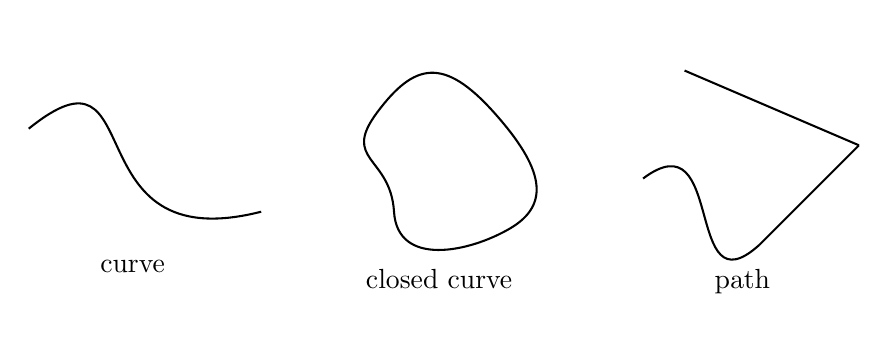
\begin{tikzpicture}[x=0.75pt,y=0.75pt,yscale=-1,xscale=1]
%uncomment if require: \path (0,476); %set diagram left start at 0, and has height of 476

%Curve Lines [id:da633375351005504] 
\draw    (96,88) .. controls (155.67,39.83) and (115.33,151.58) .. (208,128) ;
%Shape: Polygon Curved [id:ds6818018149824627] 
\draw   (264,80) .. controls (281.67,56.42) and (295.83,53.08) .. (320,80) .. controls (344.17,106.92) and (347.67,124.42) .. (328,136) .. controls (308.33,147.58) and (273.67,154.92) .. (272,128) .. controls (270.33,101.08) and (246.33,103.58) .. (264,80) -- cycle ;
%Straight Lines [id:da03683440295817464] 
\draw    (412,60) -- (496,96) ;
%Straight Lines [id:da5134672181407913] 
\draw    (448,144) -- (496,96) ;
%Curve Lines [id:da12668131694121176] 
\draw    (392,112) .. controls (432,82) and (411.33,177.08) .. (448,144) ;

% Text Node
\draw (129,150) node [anchor=north west][inner sep=0.75pt]   [align=left] {curve};
% Text Node
\draw (257,154) node [anchor=north west][inner sep=0.75pt]   [align=left] {closed curve};
% Text Node
\draw (425,154) node [anchor=north west][inner sep=0.75pt]   [align=left] {path};


\end{tikzpicture}
\end{center}
A \textbf{closed path} is a closed curve which is also a path.\par
Now suppose $\gamma$ is a path, and $f$ is a continuous function on $\gamma^*$. The integral of $f$ over $\gamma$ is defined as an integral over the parameter interval $[\alpha,\beta]$ of $\gamma$: 
$$
\oint_{\gamma}{f\left( z \right) \mathrm{d}z}=\int_{\alpha}^{\beta}{f\left( \gamma \left( t \right) \right) \gamma ^{\prime}\left( t \right) \mathrm{d}t}.
$$
We may simply write $\int f$ instead of $\oint f$ when no confusion will be made or no need to emphasize the fact that the integral is taken over path.\par
Now suppose $\gamma^*=[\alpha_1,\beta_1]$. Let $\varphi$ be a continuous mapping of $[\alpha_1,\beta_1]$ to $[\alpha,\beta]$. Then let $\gamma_1=\gamma\circ\varphi$. Observe that 
$$
\int_{\alpha _1}^{\beta _1}{f\left( \gamma _1\left( t \right) \right) \gamma _{1}^{\prime}\left( t \right) \mathrm{d}t}=\int_{\alpha _1}^{\beta _1}{f\left( \gamma \left( \varphi \left( t \right) \right) \right) \gamma ^{\prime}\left( \varphi \left( t \right) \right) \varphi ^{\prime}\left( t \right)}=\int_{\alpha}^{\beta}{f\left( \gamma \left( s \right) \right) \gamma ^{\prime}\left( s \right) \mathrm{d}s},
$$
therefore 
$$
\oint_{\gamma}{f\left( z \right) \mathrm{d}z}=\oint_{\gamma ^1}{f\left( z \right) \mathrm{d}z}.
$$
So our "reparametrization" has not changed the integral, and we shall call the path $\gamma$ and $\gamma_1$ equivalent under such circumstance.\par
We list a trivial inequality 
$$
\left| \oint_{\gamma}{f\left( z \right) \mathrm{d}z} \right|\le \left\| f \right\| _{\infty}\cdot \int_{\alpha}^{\beta}{\left| \gamma ^{\prime}\left( t \right) \right|\mathrm{d}t},
$$
where $\|f\|_\infty$ is the maximum of $|f|$ and the last integral is the \textbf{length} of $\gamma$.\par
Here are some special cases.
\begin{example}\em
(a) If $a$ is a complex number and $r>0$, then the path defined by 
$$\gamma(t)=a+re^{\mathrm{i}t}\hspace{0.5cm}(0\le t\le 2\pi)$$
is called the \textbf{positively oriented circle} with center at $a$ and radius $r$, we have 
$$
\oint_{\gamma}{f\left( z \right) \mathrm{d}z}=\mathrm{i}r\int_0^{2\pi}{f\left( a+re^{\mathrm{i}\theta} \right) e^{\mathrm{i}\theta}\mathrm{d}\theta},
$$
and the length of $\gamma$ is $2\pi r$, as expected.\par
(b) If $a$ and $b$ are complex numbers, the path $\gamma$ given by 
$$\gamma(t)=a+(b-a)t\hspace{0.5cm}(0\le t\le 1)$$
is the \textbf{oriented interval} $[a,b]$. Its length is $|b-a|$, and 
$$
\oint_{\gamma}{f\left( z \right) \mathrm{d}z}=\left( b-a \right) \int_0^1{f\left( a+\left( b-a \right) t \right) \mathrm{d}t}.
$$
If 
$$
\gamma _1=\frac{a\left( \beta -t \right) +b\left( t-\alpha \right)}{\beta -\alpha},\hspace{0.5cm}\left( t\in \left[ \alpha ,\beta \right] =\gamma ^* \right) 
$$
then $\gamma_1$ and $\gamma$ are equivalent.\par
(c) Let $\{a,b,c\}$ be an oriented triple of complex numbers, let $\Delta=\Delta(a,b,c)$ be the triangle with vertices at $a,b$ and $c$. Define 
$$
\int_{\partial \Delta}{f\left( z \right) \mathrm{d}z}=\int_{\left[ a,b \right]}{f\left( z \right) \mathrm{d}z}+\int_{\left[ b,c \right]}{f\left( z \right) \mathrm{d}z}+\int_{\left[ c,a \right]}{f\left( z \right) \mathrm{d}z}
$$
for any $f$ continuous on $\partial\Delta$. Note that if $\{a,b,c\}$ is permuted cyclically, we see that the value of $\int_{\partial\Delta}f$ is unaffected. However if $\{a,b,c\}$ is replaced by $\{a,c,b\}$, then the value of the integral differs with a sign.
\begin{center}


\tikzset{every picture/.style={line width=0.75pt}} %set default line width to 0.75pt        

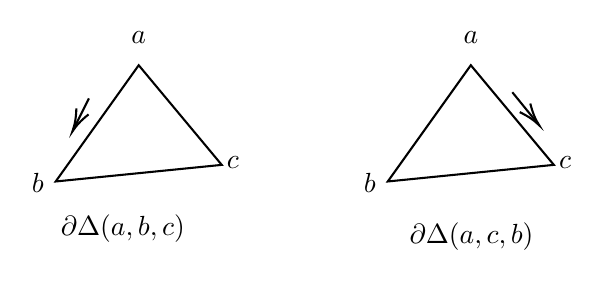
\begin{tikzpicture}[x=0.75pt,y=0.75pt,yscale=-1,xscale=1]
%uncomment if require: \path (0,476); %set diagram left start at 0, and has height of 476

%Shape: Polygon [id:ds7341302947491242] 
\draw   (216,128) -- (136,136) -- (176,80) -- cycle ;
%Straight Lines [id:da41978954017626924] 
\draw    (152,96) -- (144.89,110.21) ;
\draw [shift={(144,112)}, rotate = 296.57] [color={rgb, 255:red, 0; green, 0; blue, 0 }  ][line width=0.75]    (10.93,-3.29) .. controls (6.95,-1.4) and (3.31,-0.3) .. (0,0) .. controls (3.31,0.3) and (6.95,1.4) .. (10.93,3.29)   ;
%Shape: Polygon [id:ds08164662287981983] 
\draw   (376,128) -- (296,136) -- (336,80) -- cycle ;
%Straight Lines [id:da4173250248430085] 
\draw    (356,93) -- (367.74,107.45) ;
\draw [shift={(369,109)}, rotate = 230.91] [color={rgb, 255:red, 0; green, 0; blue, 0 }  ][line width=0.75]    (10.93,-3.29) .. controls (6.95,-1.4) and (3.31,-0.3) .. (0,0) .. controls (3.31,0.3) and (6.95,1.4) .. (10.93,3.29)   ;

% Text Node
\draw (171,62.4) node [anchor=north west][inner sep=0.75pt]    {$a$};
% Text Node
\draw (123,130.4) node [anchor=north west][inner sep=0.75pt]    {$b$};
% Text Node
\draw (217,122.4) node [anchor=north west][inner sep=0.75pt]    {$c$};
% Text Node
\draw (331,62.4) node [anchor=north west][inner sep=0.75pt]    {$a$};
% Text Node
\draw (283,130.4) node [anchor=north west][inner sep=0.75pt]    {$b$};
% Text Node
\draw (377,122.4) node [anchor=north west][inner sep=0.75pt]    {$c$};
% Text Node
\draw (137,150.4) node [anchor=north west][inner sep=0.75pt]    {$\partial \Delta ( a,b,c)$};
% Text Node
\draw (305,154.4) node [anchor=north west][inner sep=0.75pt]    {$\partial \Delta ( a,c,b)$};


\end{tikzpicture}
\end{center}
\end{example}
We now come to a theorem which plays a very important role in function theory.
\begin{theorem}
Let $\gamma$ be a closed path, let $\Omega$ be the complement of $\gamma^*$ (relative to the plane), and define 
$$
\mathrm{Ind}_{\gamma}\left( z \right) =\frac{1}{2\pi \mathrm{i}}\int_{\gamma}{\frac{\mathrm{d}\zeta}{\zeta -z}},\hspace{0.5cm}\left( z\in \Omega \right) 
$$
then $\mathrm{Ind}_\gamma$ is an integer-valued function on $\Omega$ which is constant in each component of $\Omega$ and $0$ in the unbounded component of $\Omega$.
\end{theorem}
We call $\mathrm{Ind}_\gamma(z)$ the \textbf{index} of $z$ with respect to $\gamma$. Note that $\gamma$ is compact, hence $\gamma^*$ lies in a bounded disc $D$ whose complement is connected, therefore $\Omega$ has precisely one unbounded component.
\begin{proof}
Let $[\alpha,\beta]$ be the parameter of $\gamma$, then 
$$
\mathrm{Ind}_{\gamma}\left( z \right) =\frac{1}{2\pi \mathrm{i}}\oint_{\gamma}{\frac{\mathrm{d}\zeta}{\zeta -z}}=\frac{1}{2\pi \mathrm{i}}\int_{\alpha}^{\beta}{\frac{\gamma ^{\prime}\left( s \right)}{\gamma \left( s \right) -z}\mathrm{d}s}.
$$
Note that $w/2\pi\mathrm{i}$ is an integer if and only if $e^w=1$, it suffices to show that $\varphi(\beta)=1$, where 
$$
\varphi \left( t \right) =\exp \left( \int_{\alpha}^t{\frac{\gamma ^{\prime}\left( s \right)}{\gamma \left( s \right) -z}\mathrm{d}s} \right) .
$$
Take the derivative over both sides (except possibly on a finite set $S$ that the derivative may not exist), we obtain 
$$
\varphi ^{\prime}\left( t \right) =\frac{\gamma ^{\prime}\left( t \right)}{\gamma \left( t \right) -z}\cdot \exp \left( \int_{\alpha}^t{\frac{\gamma ^{\prime}\left( s \right)}{\gamma \left( s \right) -z}\mathrm{d}s} \right) =\frac{\gamma ^{\prime}\left( t \right) \cdot \varphi \left( t \right)}{\gamma \left( t \right) -z}.
$$
Now that 
$$
\begin{aligned}
\varphi ^{\prime\prime}\left( t \right) &=\left[ \frac{\gamma ^{\prime}\left( t \right)}{\gamma \left( t \right) -z}\cdot \exp \left( \int_{\alpha}^t{\frac{\gamma ^{\prime}\left( s \right)}{\gamma \left( s \right) -z}\mathrm{d}s} \right) \right] ^{\prime}
\\
&=\frac{\gamma ^{\prime\prime}\left( t \right) \left( \gamma \left( t \right) -z \right) -\left[ \gamma ^{\prime}\left( t \right) \right] ^2}{\left( \gamma \left( t \right) -z \right) ^2}\cdot \exp \left( \int_{\alpha}^t{\frac{\gamma ^{\prime}\left( s \right)}{\gamma \left( s \right) -z}\mathrm{d}s} \right) +\left( \frac{\gamma ^{\prime}\left( t \right)}{\gamma \left( t \right) -z} \right) ^2\cdot \exp \left( \int_{\alpha}^t{\frac{\gamma ^{\prime}\left( s \right)}{\gamma \left( s \right) -z}\mathrm{d}s} \right) 
\\
&=\left( \frac{\gamma ^{\prime\prime}\left( t \right)}{\gamma \left( t \right) -z} \right) \exp \left( \int_{\alpha}^t{\frac{\gamma ^{\prime}\left( s \right)}{\gamma \left( s \right) -z}\mathrm{d}s} \right) ,
\end{aligned}
$$
therefore 
$$
\begin{aligned}
\left( \frac{\varphi \left( t \right)}{\gamma \left( t \right) -z} \right) ^{\prime}&=\left( \frac{\varphi ^{\prime}\left( t \right)}{\gamma ^{\prime}\left( t \right)} \right) ^{\prime}=\frac{\varphi ^{\prime\prime}\left( t \right) \gamma ^{\prime}\left( t \right) -\varphi ^{\prime}\left( t \right) \gamma ^{\prime\prime}\left( t \right)}{\left[ \gamma ^{\prime}\left( t \right) \right] ^2}
\\
&=\frac{1}{\left[ \gamma ^{\prime}\left( t \right) \right] ^2}\left[ \left( \frac{\gamma ^{\prime}\left( t \right) \cdot \gamma ^{\prime\prime}\left( t \right)}{\gamma \left( t \right) -z} \right) \exp \left( \int_{\alpha}^t{\frac{\gamma ^{\prime}\left( s \right)}{\gamma \left( s \right) -z}\mathrm{d}s} \right) -\frac{\gamma ^{\prime}\left( t \right) \cdot \gamma ^{\prime\prime}\left( t \right)}{\gamma \left( t \right) -z}\cdot \varphi \left( t \right) \right] =0,
\end{aligned}
$$
hence $\varphi/(\gamma-z)$ is a constant on $[\alpha,\beta]$. Since $\varphi(\alpha)=1$, we obtain 
$$
\varphi \left( t \right) =\frac{\gamma \left( t \right) -z}{\gamma \left( \alpha \right) -z},\hspace{0.5cm}\left( \alpha \le t\le \beta \right) 
$$
and since $\gamma$ is a closed path, we have $\gamma(\alpha)=\gamma(\beta)$ and hence $\varphi(\alpha)=\varphi(\beta)=1$, therefore $\mathrm{Ind}_\gamma(z)$ is an integer.\par
By Theorem 10.1.4, we have $\mathrm{Ind}_\gamma\in H(\Omega)$. Since the image of a connected set under continuous mapping is connected, we obtain $\mathrm{Ind}_\gamma$ a constant on each component of $\Omega$.\par
Finally, suppose $|z|$ is sufficiently large. Then 
$$
\left| \mathrm{Ind}_{\gamma}\left( z \right) \right|\le \int_{\gamma}{\left| \frac{1}{\zeta -z} \right|\mathrm{d}\zeta}<1,
$$
whence $\mathrm{Ind}_\gamma(z)=0$ when $z$ lies in the unbounded component of the complement of $\gamma^*$.
\end{proof}
\begin{note}\em
Now we illustrate the geometric understanding of the theorem. Suppose 
$$\lambda(t)=\int_{\alpha}^{t}\frac{\gamma^\prime(s)}{\gamma(s)-z}\mathrm{d}s.$$
Then the preceding proof shows that $2\pi\mathrm{Ind}_\gamma(z)$ is precisely the net increasing of the imaginary part of $\lambda(t)$, i.e. the net increase of the argument of $\gamma(t)-z$. If we divide this increase by $2\pi$, we obtain "the number of times that $\gamma$ winds around $z$", and this explains why the term \textbf{winding number} is used for the index.
\end{note}
 One virtue of the preceding proof is that it establishes the main properties of the index without any reference to the argument of a complex number.
 \begin{theorem}
 If $\gamma$ is the positively oriented circle with center at $a$ and radius $r$, then $\mathrm{Ind}_\gamma(z)=1$ if $|z-a|<r$, and $\mathrm{Ind}_\gamma(z)=0$ if $|z-a|>r$.
 \end{theorem}
 \begin{proof}
We take $\gamma(t)=a+re^{\mathrm{i}t}$ with $\le t\le 2\pi$. Then by Theorem  10.2.2, it suffices to show the case when $|z-a|<r$, which is 
$$
\frac{1}{2\pi \mathrm{i}}\oint_{\gamma}{\frac{\mathrm{d}\zeta}{\zeta -a}}=\frac{r}{2\pi}\int_0^{2\pi}{\left( re^{\mathrm{i}t} \right) ^{-1}\cdot e^{\mathrm{i}t}\mathrm{d}t}=1.
$$
Therefore the proof is finished.
\end{proof}
\subsection{The Local Cauchy Theorem}
There are several forms of Cauchy's theorem. They all assert that if $\gamma$ is a closed path or cycle in $\Omega$, and if $\gamma$ and $\Omega$ satisfy certain topological conditions, then the integral of every $f\in H(\Omega)$ over $\gamma$ is $0$. We shall first derive a simple local version of this which is quite sufficient for many applications. A more general global form will be established later.
\begin{theorem}
Suppose $f\in H(\Omega)$ and $F^\prime$ is continuous in $\Omega$. Then 
$$\int_\gamma F^\prime(z)\mathrm{d}z=0$$
for every closed path $\gamma\in\Omega$.
\end{theorem}
\begin{proof}
If $[\alpha,\beta]$ is the parameter interval of $\gamma$, the fundamental theorem of calculus shows that 
$$
\oint_{\gamma}{F^{\prime}\left( z \right) \mathrm{d}z}=\int_{\alpha}^{\beta}{F^{\prime}\left( \gamma \left( t \right) \right) \gamma ^{\prime}\left( t \right) \mathrm{d}t}=F\left( \gamma \left( \beta \right) \right) -F\left( \gamma \left( \alpha \right) \right) =0.
$$
This finished the proof.
\end{proof}
A simple corollary of Theorem 10.2.3 is that $\int_\gamma z^n\mathrm{d}z=0$ for all $n\in\mathbb{N}\setminus\{-1\}$ if $\gamma$ is a closed path, and $0\notin\gamma^*$ if $n<-1$. This is due to $z^n$ is the derivative of $z^{n+1}/(n+1)$ when $n\ne -1$. The condition that $n=-1$ has been dealt with in the previous section.\par
Now we introduce the following \textbf{Cauchy's Theorem in a triangle}.
\begin{theorem}
Suppose $\Delta$ is a closed triangle in a plane open set $\Omega$, $p\in\Omega$, and $f$ is continuous on $\Omega$ such that $f\in H(\Omega\setminus\{p\})$. Then 
$$\int_{\partial\Delta}f(z)\mathrm{d}z=0.$$
\end{theorem}
\begin{proof}
We assume that $p\notin\Delta$ first. Suppose the three vertices of $\Delta$ are $a,b$ and $c$. Let $a^\prime$, $b^\prime$ and $c^\prime$ be the midpoint of the opposite side relative to $a$, $b$ and $c$, then define four triangles 
$$
\Delta ^1=\Delta \left\{ a,c^{\prime},b^{\prime} \right\} ,\Delta ^2=\Delta \left\{ b,a^{\prime},c^{\prime} \right\} ,\Delta ^3=\Delta \left\{ c,b^{\prime},a^{\prime} \right\} ,\Delta ^4=\Delta \left\{ a^{\prime},b^{\prime},c^{\prime} \right\}. 
$$
Now if $J$ is the value of $\oint_{\partial\Delta}f(z)\mathrm{d}z$, then 
$$
J=\sum_j{\int_{\partial \Delta ^j}{f\left( z \right) \mathrm{d}z}}.
$$
Clearly there exists some triangle, say $\Delta_1\in\{\Delta^j\}_j$, such that 
$$
\left| \int_{\partial \Delta ^i}{f\left( z \right) \mathrm{d}z} \right|>\left| \frac{J}{4} \right|.
$$
Repeat the previous operation on $\Delta_1$, we obtain a sequence of triangles $\Delta \supset \Delta _1\supset \cdots \supset \Delta _n\supset \cdots $ such that the length of $\partial\Delta_n$ is $2^{-n}L$, where $L$ is the length of $\partial\Delta$. Therefore 
$$
\left| J \right|\le 4\left| \int_{\partial \Delta _1}{f\left( z \right) \mathrm{d}z} \right|\le 4^2\left| \int_{\partial \Delta _2}{f\left( z \right) \mathrm{d}z} \right|\le \cdots \le 4^n\left| \int_{\partial \Delta _n}{f\left( z \right) \mathrm{d}z} \right|.
$$
Since each $\Delta_k$ is compact, there exists a unique $z_0\in\bigcap_{n}\Delta_n$. Since $p\notin\Delta$, $f$ is differentiable at $z_0$. Let $\varepsilon>0$. Then there corresponds $r>0$ such that 
$$
\left| f\left( z \right) -f\left( z_0 \right) -f^{\prime}\left( z \right) \left( z-z_0 \right) \right|\le \varepsilon \left| z-z_0 \right|,\hspace{0.5cm}\left( \left| z-z_0 \right|<r \right) 
$$
whence 
$$
\left| \int_{\partial \Delta _n}{f\left( z \right) \mathrm{d}z} \right|=\left| \int_{\partial \Delta _n}{\left[ f\left( z \right) -f\left( z_0 \right) -f^{\prime}\left( z \right) \left( z-z_0 \right) \right] \mathrm{d}z} \right|\le \varepsilon \cdot 2^{-n}L\cdot r.
$$
Since there exists some large $n$ such that $r<2^{-n}L$, we obtain 
$$
\left| \int_{\partial \Delta _n}{f\left( z \right) \mathrm{d}z} \right|\le \varepsilon \cdot \left( 2^{-n}L \right) ^2=\frac{\varepsilon L^2}{4^n}.
$$
Therefore 
$$
J=\left| \int_{\partial \Delta _n}{f\left( z \right) \mathrm{d}z} \right|\le \frac{\varepsilon L^2}{4^n}\rightarrow 0,
$$
hence $J=0$ and the proof is finished.\par
Now suppose $p$ is a vertex of $\Delta$, say $p=a$. Then we may divide the triangle $\Delta$ into three small triangles, $\Delta \left( a,x,y \right) ,\Delta \left( x,b,y \right) ,\Delta \left( b,c,y \right) $, as shown below:
\begin{center}


\tikzset{every picture/.style={line width=0.75pt}} %set default line width to 0.75pt        

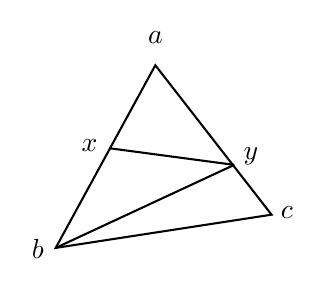
\begin{tikzpicture}[x=0.75pt,y=0.75pt,yscale=-1,xscale=1]
%uncomment if require: \path (0,476); %set diagram left start at 0, and has height of 476

%Shape: Polygon [id:ds944599867727798] 
\draw   (216,136) -- (168,224) -- (272,208) -- cycle ;
%Straight Lines [id:da763895858654525] 
\draw    (194,176) -- (254,184) ;
%Straight Lines [id:da18568190298138365] 
\draw    (168,224) -- (254,184) ;

% Text Node
\draw (211,118.4) node [anchor=north west][inner sep=0.75pt]    {$a$};
% Text Node
\draw (155,218.4) node [anchor=north west][inner sep=0.75pt]    {$b$};
% Text Node
\draw (275,202.4) node [anchor=north west][inner sep=0.75pt]    {$c$};
% Text Node
\draw (179,170.4) node [anchor=north west][inner sep=0.75pt]    {$x$};
% Text Node
\draw (257,174.4) node [anchor=north west][inner sep=0.75pt]    {$y$};


\end{tikzpicture}
\end{center}
therefore 
$$
\int\limits_{\partial \Delta}{f\left( z \right) \mathrm{d}z}=\int\limits_{\partial \Delta \left( a,x,y \right)}{f\left( z \right) \mathrm{d}z}+\int\limits_{\partial \Delta \left( x,b,y \right)}{f\left( z \right) \mathrm{d}z}+\int\limits_{\partial \Delta \left( b,c,y \right)}{f\left( z \right) \mathrm{d}z}=\int\limits_{\partial \Delta \left( a,x,y \right)}{f\left( z \right) \mathrm{d}z}.
$$
Then since $f$ is continuous on $\Delta$, we may let $x$ and $y$ arbitrarily close to $a$, therefore the integral $\int_{\partial\Delta(a,x,y)}f(z)\mathrm{d}z$ converges to zero, and hence $\int_{\partial\Delta}f(z)\mathrm{d}z=0$ holds for this condition.\par
Now suppose $p$ lies in the interior of $\Delta$, such condition may be easily deduced into the condition of two previous conditions, therefore our proof is finished.
\end{proof}
Our next theorem is the \textbf{Cauchy's theorem in a convex open set}.
\begin{theorem}
Let $\Omega$ be a convex open set, $p\in\Omega$, $f$ is continuous on $\Omega$ and $f\in H(\Omega\setminus\{p\})$. Then 
$$\int_\gamma f(z)\mathrm{d}z=0$$
for all closed path $\gamma\in\Omega$.
\end{theorem}
\begin{proof}
Let $a\in\Omega$. Since $\Omega$ is convex, the line $[a,z]$ lies in $\Omega$ for all $z\in\Omega$. Therefore we may define the integral 
$$
F\left( z \right) =\int_{\left[ a,z \right]}{f\left( \zeta \right) \mathrm{d}\zeta}.\hspace{0.5cm}\left( z\in \Omega \right) 
$$
Now consider $z_0\in\Omega$. Since $a,z$ and $z_0$ forms a triangle, we apply Theorem 10.3.2 to obtain 
$$
\int_{\partial \Delta}{f\left( \zeta \right) \mathrm{d}\zeta}=\int_{\left[ a,z \right]}{f\left( \zeta \right) \mathrm{d}\zeta}+\int_{\left[ z,z_0 \right]}{f\left( \zeta \right) \mathrm{d}\zeta}+\int_{\left[ z_0,a \right]}{f\left( \zeta \right) \mathrm{d}\zeta}=0,
$$
hence 
$$
\int_{\left[ z_0.z \right]}{f\left( \zeta \right) \mathrm{d}\zeta}=\int_{\left[ a,z \right]}{f\left( \zeta \right) \mathrm{d}\zeta}-\int_{\left[ a,z_0 \right]}{f\left( \zeta \right) \mathrm{d}\zeta}.
$$
Therefore 
$$
\frac{F\left( z \right) -F\left( z_0 \right)}{z-z_0}-f\left( z_0 \right) =\frac{1}{z-z_0}\int_{\left[ z_0,z \right]}{f\left( \zeta \right) \mathrm{d}\zeta}-f\left( z_0 \right) =\frac{1}{z-z_0}\int_{\left[ z_0,z \right]}{\left[ f\left( \zeta \right) -f\left( z_0 \right) \right] \mathrm{d}\zeta}.
$$
Since $f$ is continuous in $\Omega$, for all $\varepsilon>0$ there exists some $\delta>0$, such that when $|\zeta-z_0|<\delta$ we have $|f(\zeta)-f(z_0)|<\varepsilon$. Now let $z_0\to z$, we have 
$$
\left| \frac{F\left( z \right) -F\left( z_0 \right)}{z-z_0}-f\left( z_0 \right) \right|\le \frac{1}{\left| z-z_0 \right|}\cdot \varepsilon \cdot \left| z-z_0 \right|=\varepsilon ,
$$
therefore $F^\prime(z_0)=f(z_0)$. Since $z_0$ is arbitrarily chosen, we may conclude that 
$$
\int_{\gamma}{f\left( z \right) \mathrm{d}z}=\int_{\gamma}{F^{\prime}\left( z \right) \mathrm{d}z}=0,
$$
where the last equality follows from theorem 10.3.1.
\end{proof}
\begin{theorem}
Let $\Omega$ be an open convex set, $f\in H(\Omega)$. Suppose $\gamma$ is a closed path, $z\in\Omega$ and $z\notin\gamma^*$, then 
$$
f\left( z \right) \cdot \mathrm{Ind}_{\gamma}\left( z \right) =\frac{1}{2\pi \mathrm{i}}\int_{\gamma}{\frac{f\left( \zeta \right)}{\zeta -z}\mathrm{d}\zeta}.
$$
\end{theorem}
\begin{proof}
We consider the function 
$$
g\left( \zeta \right) =\begin{cases}
	\frac{f\left( \zeta \right) -f\left( z \right)}{\zeta -z},\zeta \in \Omega \setminus \left\{ z \right\} ,\\
	f^{\prime}\left( z \right) ,\zeta =z.\\
\end{cases}
$$
Then clearly $g^\prime(\zeta)$ is holomorphic, therefore apply Theorem 10.3.3, we obtain 
$$
0=\frac{1}{2\pi \mathrm{i}}\int_{\gamma}{g\left( \zeta \right) \mathrm{d}\zeta}=\frac{1}{2\pi \mathrm{i}}\int_{\gamma}{\frac{f\left( \zeta \right) -f\left( z \right)}{\zeta -z}\mathrm{d}\zeta}=\frac{1}{2\pi \mathrm{i}}\int_{\gamma}{\frac{f\left( \zeta \right)}{\zeta -z}\mathrm{d}\zeta}-f\left( z \right) \cdot \frac{1}{2\pi \mathrm{i}}\int_{\gamma}{\frac{\mathrm{d}\zeta}{\zeta -z}},
$$
hence 
$$
f\left( z \right) \cdot \mathrm{Ind}_{\gamma}\left( z \right) =f\left( z \right) \cdot \frac{1}{2\pi \mathrm{i}}\int_{\gamma}{\frac{\mathrm{d}\zeta}{\zeta -z}}=\frac{1}{2\pi \mathrm{i}}\int_{\gamma}{\frac{f\left( \zeta \right)}{\zeta -z}\mathrm{d}\zeta}.
$$
This finished the proof.
\end{proof}
We now come to an easy corollary of Theorem 10.3.4, which answered the question about the converse of Theorem 10.1.2.
\begin{theorem}
Suppose $\Omega$ is an open set. Let $f$ be a holomorphic function on $\Omega$, then $f$ is representable by power series in $\Omega$.
\end{theorem}
\begin{proof}
Since $\omega$ is open, for all $a\in\Omega$ there exists an open disc $D(a,R)$ such that $D(a,R)\subset\Omega$. Now take $\gamma$ an oriented circle centered at $a$ with radius $r<R$, then 
$$
f\left( z \right) =f\left( z \right) \cdot \mathrm{Ind}_{\gamma}\left( z \right) =\frac{1}{2\pi \mathrm{i}}\int_{\gamma}{\frac{f\left( \zeta \right)}{\zeta -z}\mathrm{d}\zeta}.\hspace{0.5cm}\left( z\in D\left( a,r \right) \right) 
$$
However by Theorem 10.1.4 with $X=2\pi$, $\mathrm{d}\mu(\zeta)=f(\gamma(z))\gamma^\prime(z)\mathrm{d}z$ and $\varphi(z)=\gamma(z)$, we conclude that $f(z)$ is representable by a power series in $D(a,R)$. Since the representation is valid for every $z\in D(a,R)$, the proof is complete.
\end{proof}
The Cauchy theorem has a useful reverse, which is usually called the \textbf{Morera's theorem}: 
\begin{theorem}
Suppose $f$ is a complex function in an open set $\Omega$ such that 
$$\int_{\partial\Delta}f(z)\mathrm{d}z=0$$
for all triangle $\Delta\subset\Omega$, then $f\in H(\Omega)$.
\end{theorem}
\begin{proof}
Let $V$ be a convex subset of $\Omega$, then by the proof of Theorem 10.3.3 we may construct a function $F$ such that $F\in H(\Omega)$ and $F^\prime=f$. Therefore $f$ is the derivative of a holomorphic function, which is also holomorphic.
\end{proof}
\subsection{The Power Series Representation}
The fact that every holomorphic function is locally the sum of a convergent power series has a large number of interesting consequences. A few of these are developed in this section.
\begin{theorem}
Suppose $\Omega$ is a region, $f\in H(\Omega)$, and $Z(f)=\{a\in\Omega:f(a)=0\}$. Then either $Z(f)=\Omega$, or $Z(f)$ has no limit point in $\Omega$. In the latter case there corresponds to each $a\in Z(f)$ a unique positive integer $m=m(a)$ such that 
$$f(z)=(z-a)^mg(z),\hspace{0.5cm}(z\in\Omega)$$
where $g\in H(\Omega)$ and $g(a)\ne 0$. Furthermore, $Z(f)$ is at most countable.
\end{theorem}
\begin{proof}
Let $A$ be the set of all limit points of $Z(f)$. Now suppose $a\in Z(f)$, choose $r>0$ such that 
$$
f\left( z \right) =\sum_{n=0}^{\infty}{c_n\left( z-a \right) ^n},\hspace{0.5cm}z\in D\left( a,r \right) .
$$
Now there are two possibilities: $c_n=0$ for all $n\in\mathbb{N}$, or there exists a minimum $m\in\mathbb{N}$ such that $c_m\ne 0$. Now if it is the latter case, we define 
$$
g\left( z \right) =\begin{cases}
	\frac{f\left( z \right)}{\left( z-a \right) ^m},z\in \Omega \setminus \left\{ a \right\} ,\\
	c_m,z=a.\\
\end{cases}
$$
whence 
$$
f\left( z \right) =\left( z-a \right) ^mg\left( z \right) ,\hspace{0.5cm}g\in H\left( \Omega \setminus \left\{ a \right\} \right) .
$$
But observe that 
$$
f\left( z \right) =\left( z-a \right) ^mg\left( z \right) =\sum_{n=0}^{\infty}{c_n\left( z-a \right) ^n}=\sum_{k=0}^{\infty}{c_{m+k}\left( z-a \right) ^{m+k}},
$$
we have 
$$
g\left( z \right) =\sum_{k=0}^{\infty}{c_{n+k}\left( z-a \right) ^k},\hspace{0.5cm}z\in D\left( a,r \right) .
$$
Therefore $g\in H(\Omega)$. Since $g$ is continuous on $\Omega$, in particular continuous at $a$, we have $a$ an isolated point in $Z(f)$.\par
Now suppose $a\in A$. Then the first case, i.e. $c_n=0$ for all $n\in\mathbb{N}$, must occur. Therefore $f$ is a constant and hence $a$ is an interior of $A$, therefore $A$ is open. Now consider $B=\Omega\setminus A$, which, by definition of $A$, is also open. Therefore $\Omega$ is the disjoint union of two open sets, and by the connectivity of $\Omega$ we have either $A=\Omega$ and $B=\Omega$. If $A=\Omega$, then $Z(f)=\Omega$. If $B=\Omega$, then $A=\emptyset$, hence $Z(f)$ has at most finite many points in a compact subset of $\Omega$. Since $\Omega$ is $\sigma$-compact, we have $Z(f)$ contains at most countably many points.
\end{proof}
\begin{note}\em
(a) The integer $m$ in Theorem 10.4.1 is called the \textbf{order} of the zero which $f$ has at the point $a$. Clearly $Z(f)=\Omega$ if and only if $f$ is identically $0$ in $\Omega$. We call $Z(f)$ the \textbf{zero set} of $f$. Analogous results hold of course for the set of $\alpha$-points of $f$, i.e. the zero set of $f-\alpha$, where $\alpha$ is any complex number.\par
(b) The theorem may fail if the condition $\Omega$ is connected is omitted. For example, consider $\Omega=\Omega_1\cup\Omega_2$, where $\Omega_1$ and $\Omega_2$ are disjoint connected open sets. Put $f(z)=1$ for $z\in\Omega_1$ and $f(z)=0$ for $z\in\Omega_2$.
\end{note}
\begin{corollary}
If $f$ and $g$ are holomorphic functions in a region $\Omega$ and if $f(z)=g(z)$ for all $z$ in some set which has a limit point $\Omega$, then $f(z)=g(z)$ for all $z\in\Omega$.
\end{corollary}
\begin{proof}
Let $h(z)=f(z)-g(z)$ and $Z(h)$ defined similar to the way in Theorem 10.4.1. Then $Z(h)$ contains a limit point in $\Omega$, hence $Z(h)=\Omega$ by Theorem 10.4.1. Therefore $f(z)-g(z)=0$ for all $z\in\Omega$, which is $f(z)=g(z)$ for all $z\in\Omega$.
\end{proof}
\begin{definition}
If $a\in\Omega$ and $f\in H(\Omega\setminus\{a\}$, then $f$ is said to have an \textbf{isolated singularity} at the point $a$. If $f$ can be so defined at $a$ that the extended function is holomorphic in $\Omega$, the singularity is said to be \textbf{removable}.
\end{definition}
We have the following theorem for removable singularities:
\begin{theorem}
Suppose $f\in H(\Omega\setminus\{a\})$ and $f$ is bounded in $D^\prime(a,r)$ for some $r>0$. Then $f$ has a removable singularity at $a$.
\end{theorem}
\begin{proof}
We define the function 
$$
h\left( z \right) =\begin{cases}
	\left( z-a \right) ^2f\left( z \right) ,z\in \Omega \setminus \left\{ a \right\} ,\\
	0,z=a,\\
\end{cases}
$$
then by the assumption that $f$ is bounded, we have 
$$
h^{\prime}\left( a \right) =\lim_{z\rightarrow a} \frac{h\left( z \right) -h\left( a \right)}{z-a}=\lim_{z\rightarrow a} \frac{\left( z-a \right) ^2f\left( z \right)}{z-a}=\lim_{z\rightarrow a} \left( z-a \right) f\left( z \right) =0.
$$
Clearly $h$ is differentiable at every point of $\Omega\setminus\{a\}$, then $h$ is holomorphic on $\Omega$. Therefore suppose 
$$
h\left( z \right) =\sum_{n=2}^{\infty}{c_n\left( z-a \right) ^n},\hspace{0.5cm}z\in D\left( a,r \right) ,
$$
we have 
$$
f\left( z \right) =\frac{h\left( z \right)}{\left( z-a \right) ^2}=\sum_{n=0}^{\infty}{c_{n+2}\left( z-a \right) ^n}
$$
by defining $f(a)=c_2$. Therefore $f$ is representable by power series in $D(a,r)$, hence holomorphic.
\end{proof}
\begin{theorem}
If $a\in\Omega$ and $f\in H(\Omega\setminus\{a\})$, then one of the following conditions must be true:\par
(a) $f$ has a removable singularity.\par
(b) There exists $m\in\mathbb{N}$ that $m\ge 1$ and $c_1,\cdots,c_m\in\mathbb{C}$ such that 
$$
f\left( z \right) -\sum{\frac{c_k}{\left( z-a \right) ^k}}
$$
has a removable singularity.\par
(c) If $r>0$ and $D(a,r)\subset\Omega$, then $f(D^\prime(a,r))$ is dense in $\mathbb{C}$.
\end{theorem}
\begin{proof}
Suppose that (c) is false. Then there exists some $r>0$ and $\delta>0$, and for some $w\in\mathbb{C}$ such that $|f(z)-w|>\delta$ for all $z\in D^\prime(a,r)$. Let us now write $D$ for $D(a,r)$ and $D^\prime$ for $D^\prime$. Define 
$$
g\left( z \right) =\frac{1}{f\left( z \right) -w},\hspace{0.5cm}z\in D^{\prime}\left( a,r \right) .
$$
Clearly $|g|\le 1/\delta$, therefore by Theorem 10.4.4 we obtain $a$ is a removable singularity of $g$, and we may suppose $g\in H(D)$.\par
If $g(a)\ne 0$, then $f(a)$ is finite. Therefore $f$ is finite on $D$ and hence by Theorem 10.4.4 we obtain $a$ is a removable singularity of $f$, which is condition (a).\par
If $g(a)=0$, then suppose $a$ is a zero of order $m\ge 1$. By Theorem 10.4.1, there exists some $g_1(z)\in H(D)$ with $g_1(a)\ne 0$ such that 
$$
g\left( z \right) =\left( z-a \right) ^mg_1\left( z \right) ,\hspace{0.5cm}z\in D\left( a,r \right) .
$$
Now that $g_1(a)\ne 0$, we may define $h(z)=1/g_1(z)$ for $z\in D$, which is clearly a holomorphic function. Now that 
$$
f\left( z \right) -w=\frac{1}{g\left( z \right)}=\frac{1}{\left( z-a \right) ^mg_1\left( z \right)}=\frac{h\left( z \right)}{\left( z-a \right) ^m}.
$$
However $h\in H(D)$, therefore $h$ may be represented by power series in $D$ as follows: 
$$
h\left( z \right) =\sum_{n=0}^{\infty}{b_n\left( z-a \right) ^n},\hspace{0.5cm}z\in D^{\prime}\left( a,r \right) .
$$
Therefore 
$$
f\left( z \right) -w=\frac{1}{\left( z-a \right) ^m}\sum_{n=0}^{\infty}{b_n\left( z-a \right) ^n},
$$
and hence 
\begin{small}
$$
f\left( z \right) -\sum_{k=1}^m{\frac{b_{m-k}}{\left( z-a \right) ^k}}=w+\sum_{n=0}^{\infty}{b_n\left( z-a \right) ^{n-m}}-\sum_{k=1}^m{b_{m-k}\left( z-a \right) ^{-k}}=w+\sum_{n=m}^{\infty}{b_n\left( z-a \right) ^n}\in H\left( D^{\prime} \right) .
$$
\end{small}
Therefore the condition (b) is true.
\end{proof}
\begin{note}\em
In case (b), $f$ is said to have a \textbf{pole of order $m$} at $a$. The function $\sum c_k(z-a)^{-k}$ is called the \textbf{principal part} of $f$ at $a$.\par
In case (c), $f$ is said to have a \textbf{essential singularity} at $a$. A statement equivalent to (c) is that to each $w\in\mathbb{C}$ there corresponds a sequence $\{z_n\}$ such that $z_n\to a$ and $f(z_n)\to w$ as $n\to\infty$.
\end{note}
We now exploit the fact that the restriction of a power series $\sum c_n(z-a)^n$ to a circle with center at $a$ is a trigonometric series.
\begin{theorem}
If 
$$
f\left( z \right) =\sum_{n=0}^{\infty}{c_n\left( z-a \right) ^n},\hspace{0.5cm}z\in D\left( a,R \right) ,
$$
and if $0<r<R$, then 
$$
\sum_{n=0}^{\infty}{\left| c_n \right|^2r^{2n}}=\frac{1}{2\pi}\int_{-\pi}^{\pi}{\left| f\left( a+re^{\mathrm{i}\theta} \right) \right|^2\mathrm{d}\theta}.
$$
\end{theorem}
\begin{proof}
We have 
$$
f\left( a+re^{\mathrm{i}\theta} \right) =\sum_{n=0}^{\infty}{c_nr^ne^{\mathrm{i}n\theta}}.
$$
For $r<R$, the series converges uniformly on $[-\pi,\pi]$. Therefore by the Inversion formula we have 
$$
c_nr^n=\frac{1}{2\pi}\int_{-\pi}^{\pi}{f\left( a+re^{\mathrm{i}\theta} \right) e^{-\mathrm{i}n\theta}\mathrm{d}\theta},
$$
and hence 
$$
\sum_{n=0}^{\infty}{\left| c_n \right|^2r^{2n}}=\frac{1}{2\pi}\int_{-\pi}^{\pi}{\left| f\left( a+re^{\mathrm{i}\theta} \right) \right|^2\mathrm{d}\theta}
$$
by Parseval identity.
\end{proof}
Here are some consequences:
\begin{theorem}{\textbf{(Liouville)}}
Every bounded entire function is constant.
\end{theorem}
\begin{proof}
Let $f$ be an entire function and $|f(z)|<M$ for all $z\in\mathbb{C}$. Suppose $f(z)=\sum c_nz^n$ for some $c_n\in\mathbb{C}$, then by Theorem 10.4.6 we have 
$$
\sum_{n=0}^{\infty}{\left| c_n \right|^2r^{2n}}\le M^2
$$
for all $r\in\mathbb{C}$, therefore $c_n=0$ for all $n\ge 1$, and hence $f$ is a constant.
\end{proof}
\begin{theorem}{\textbf{(The Maximum Modulus Theorem)}}
Suppose $\Omega$ is a region, $f\in H(\Omega)$, and $\overline{D}(a,r)\subset\Omega$. Then 
$$
\left| f\left( a \right) \right|\le \max_{\theta} \left| f\left( a+e^{\mathrm{i}\theta} \right) \right|,
$$
and the equality holds if and only if $f$ is a constant.
\end{theorem}
\begin{proof}
Suppose $\left| f\left( a+e^{\mathrm{i}\theta} \right) \right|\le \left| f\left( a \right) \right|$ for all $\theta$. Then 
$$
\sum_{n=0}^{\infty}{\left| c_n \right|^2r^{2n}}\le \left| f\left( a \right) \right|^2=c_{0}^{2},
$$
which implies $c_n=0$ for all $n\ge 1$ and hence $f$ a constant.
\end{proof}
\begin{corollary}
Under the same hypothesis of Theorem 10.4.8, we have 
$$
\left| f\left( a \right) \right|\ge \min_{\theta} \left| f\left( a+e^{\mathrm{i}\theta} \right) \right|
$$
if $f$ has no zero in $D(a,r)$.
\end{corollary}
\begin{proof}
The condition is trivial if $f(a+e^{\mathrm{i}\theta})=0$ for some $\theta$. Otherwise consider $1/f$, which is holomorphic since $f$ has no zeros in $D(a,r)$. Apply the maximum modulus theorem on $1/f$, we have 
$$
\left| \frac{1}{f\left( a \right)} \right|\le \max_{\theta} \left| \frac{1}{f\left( a+e^{\mathrm{i}\theta} \right)} \right|,
$$
which is 
$$
\left| f\left( a \right) \right|\ge \min_{\theta} \left| f\left( a+e^{\mathrm{i}\theta} \right) \right|.
$$
This completes the proof.
\end{proof}
\begin{theorem}{\textbf{(Fundamental Theorem of Algebra)}}
If $n$ is a positive number and 
$$
P\left( z \right) =z^n+a_{n-1}z^{n-1}+\cdots +a_1z+a_0,
$$
where $a_i\in\mathbb{C}$ for all $i=0,1,2,\cdots,n-1$, then $P$ has precisely $n$ zeros (up to multiplicities) in the plane.
\end{theorem}
\begin{proof}
We first obverse that 
$$
\left| P\left( z \right) \right|\ge \left| z \right|^n-\left| a_{n-1} \right|\cdot \left| z \right|^{n-1}-\cdots -\left| a_1 \right|\cdot \left| z \right|-\left| a_0 \right|=\left| z \right|^n\cdot \left( 1-\left| \frac{a_{n-1}}{z} \right|-\cdots -\left| \frac{a_0}{z^n} \right| \right) \rightarrow \infty 
$$
as $|z|\to\infty$, therefore we may pick some large $r$ such that $|P(re^{\mathrm{i}\theta})>|P(0)|$. Now suppose there are no zeros of $P$ on $\mathbb{C}$, then $1/P$ is entire. Hence apply the maximum modulus theorem to $1/P$, we have 
$$
\left| f\left( 0 \right) \right|\le \max_{\theta} \left| f\left( re^{\mathrm{i}\theta} \right) \right|,
$$
which is a contradiction. Therefore $P$ has at least one zero. Suppose now $P(z_1)=0$, then there exists some $P_1$ such that $P_1(z_1)\ne 0$, and $P(z)=(z-z_1)P_1(z)$. Now the theorem is proved via induction.
\end{proof}
\begin{note}\em
This theorem contains the fact that $\mathbb{C}$ is \textbf{algebraically closed}, i.e. every nonconstant polynomial with complex coefficients has at least one complex zero.
\end{note}
\begin{theorem}{\textbf{(Cauchy's Estimates)}}
If $f\in H(D(a,R))$ and $|f(z)|\le M$ for all $z\in D(a,R)$, then 
$$|f^{(n)}(a)|\le\frac{n!M}{R^n}.\hspace{0.5cm}(n=1,2,3,\cdots)$$
\end{theorem}
\begin{proof}
By Cauchy's Formula we have 
$$
f\left( z \right) =\frac{1}{2\pi \mathrm{i}}\oint_{D\left( a,R \right)}{\frac{f\left( \zeta \right)}{\zeta -z}\mathrm{d}\zeta}.
$$
Now observe that 
$$
\frac{f\left( z \right) -f\left( z_0 \right)}{z-z_0}=\frac{1}{2\pi \mathrm{i}\cdot \left( z-z_0 \right)}\int_{D\left( a,R \right)}{\left( \frac{f\left( \zeta \right)}{\zeta -z}-\frac{f\left( \zeta \right)}{\zeta -z_0} \right) \mathrm{d}\zeta}=\frac{1}{2\pi \mathrm{i}}\int_{D\left( a,R \right)}{\frac{f\left( \zeta \right)}{\left( \zeta -z \right) \left( \zeta -z_0 \right)}\mathrm{d}\zeta},
$$
we conclude that 
$$
f^{\prime}\left( z \right) =\lim_{z\rightarrow z_0} \frac{f\left( z \right) -f\left( z_0 \right)}{z-z_0}=\frac{1}{2\pi \mathrm{i}}\int_{D\left( a,R \right)}{\frac{f\left( \zeta \right)}{\left( \zeta -z \right) ^2}\mathrm{d}\zeta}.
$$
Therefore by induction we have  
$$
f^{\left( n \right)}\left( z \right) =\frac{n!}{2\pi \mathrm{i}}\int_{D\left( a,R \right)}{\frac{f\left( \zeta \right)}{\left( \zeta -z \right) ^{n+1}}\mathrm{d}\zeta}.
$$
Hence 
$$
\left| f^{\left( n \right)}\left( a \right) \right|\le \frac{n!}{2\pi}\int_{D\left( a,R \right)}{\left| \frac{f\left( \zeta \right)}{\left( \zeta -a \right) ^{n+1}} \right|\mathrm{d}\zeta}=\frac{n!}{2\pi}\int_0^{2\pi}{\left| \frac{f\left( a+re^{\mathrm{i}\theta} \right)}{r^{n+1}\cdot e^{\mathrm{i}\left( n+1 \right) \theta}} \right|\mathrm{d}\theta}\le \frac{n!M}{R^n},
$$
which finished the proof.
\end{proof}
\begin{note}\em
To see that the inequality in Theorem 10.4.11 can't be improved, take $a=0$, $R=1$ and $f(z)=z^n$.
\end{note}
\begin{definition}
A sequence $\{f_j\}$ of functions in $\Omega$ is said to be \textbf{converge to $f$ uniformly on compact subsets of $\Omega$} if to every compact subset $K\subset\Omega$ and to every $\varepsilon>0$, there corresponds an $N=N(K,\varepsilon)$ such that $|f_j(z)-f(z)|<\varepsilon$ for all $z\in K$ if $j>N$.
\end{definition}
For instance, the function $f(z)=z^n$ converges uniformly on compact subsets of $D(0,1)$, but not uniformly on $D(0,1)$.\par
It is uniform convergence on compact subsets which arises most naturally in connection with limit operations on holomorphic functions. The term \textbf{almost uniform convergence} is sometimes used for this concept.
\begin{theorem}
Suppose $f_j\in H(\Omega)$ for $j=1,2,3,\cdots$, and $f_j\to f$ uniformly on compact subsets of $\Omega$. Then $f\in H(\Omega)$, and $f^\prime_j\to f^\prime$ uniformly on compact subsets of $\Omega$.
\end{theorem}
\begin{proof}
We first show that $f\in H(\Omega)$. Since $f_j\in H(\Omega)$, for any compact triangle $\Delta\subset\Omega$, we have 
$$
\int_{\partial \Delta}{f\left( z \right) \mathrm{d}z}=\lim_{j\rightarrow \infty} \int_{\partial \Delta}{f_j\left( z \right) \mathrm{d}z}=0,
$$
therefore by Morera's theorem we have $f\in H(\Omega)$.\par
Now let $K$ be compact subset of $\Omega$. Then there exists some $R>0$ such that to each $z\in K$, the disc $\overline{D}(z,R)$ is compact in $\Omega$. Now to each $z\in K$ apply Cauchy's estimates, we have 
$$
\left| f^{\prime}\left( z \right) -f_{j}^{\prime}\left( z \right) \right|\le \frac{1}{R}\cdot \mathop {\mathrm{sup}} \limits_{z\in \overline{D}\left( z,R \right)}\left| f\left( z \right) -f_j\left( z \right) \right|\rightarrow 0,\hspace{0.5cm}\left( j\rightarrow \infty \right) 
$$
therefore $f_j^\prime\to f_j$ uniformly on $K$.
\end{proof}
An immediate consequence of Theorem 10.4.13 is that, under the same hypothesis, we have $f_j^{(n)}\to f^{(n)}$ uniformly, as $j\to\infty$, on every compact subset of $\Omega$, and for every positive integer $n$. Compare to the situation on the real line, where sequences of infinitely differentiable functions can converge uniformly to nowhere differentiable functions!
\subsection{The Open Mapping Theorem}
Consider the following problem: If $\Omega$ is a region and $f\in H(\Omega)$, what can we say about $f(\Omega)$? Indeed, $f(\Omega)$ is either a region or a point. This important property will be developed in this section, and we shall answer it with a more detailed theorem.
\begin{lemma}\em
If $f\in H(\Omega)$ and $g$ is defined on $\Omega\times\Omega$ by 
$$
g\left( z,w \right) =\begin{cases}
	\frac{f\left( z \right) -f\left( w \right)}{z-w},w\ne z,\\
	f^{\prime}\left( z \right) ,w=z,\\
\end{cases}
$$
then $g$ is continuous in $\Omega\times\Omega$.
\end{lemma}
\begin{proof}
The only points at which the continuity of $g$ is possibly in doubt is $z=w$. Now fix $a\in\Omega$, then there exists some $r>0$ such that for all $\zeta\in\Omega$, we have $|f^\prime(\zeta)-f^\prime(z)|<\varepsilon$. Now take $z,w\in D(a,r)$, we have 
$$
\left| g\left( z,w \right) -g\left( a,a \right) \right|=\left| \frac{f\left( z \right) -f\left( w \right)}{z-w}-f^{\prime}\left( a \right) \right|\le \int_0^1{\left| f^{\prime}\left( \left( 1-t \right) z+tw \right) -f^{\prime}\left( a \right) \right|\mathrm{d}z}<\varepsilon ,
$$
whence $f$ is continuous at the point $(a,a)$, which finished the proof.
\end{proof}
\begin{theorem}
Suppose $\varphi\in H(\Omega)$, $z_0\in\Omega$ and $\varphi^\prime(z_0)\ne 0$. Then $\Omega$ contains a neighborhood $V$ of $z_0$ such that \par
(i) $\varphi$ is one-to-one in $V$;\par
(ii) $W=\varphi(V)$ is an open set, and \par
(iii) If $\psi:W\to V$ is defined by $\psi(\varphi(z))=z$, then $\psi\in H(W)$.
\end{theorem}
\begin{proof}
(i) Apply Lemma 10.5.1 to $\varphi$, we obtain that there exists some neighborhood $V$ of $z_0$ such that 
$$
\left| \varphi \left( z_1 \right) -\varphi \left( z_2 \right) \right|\ge \frac{1}{2}\left| \varphi ^{\prime}\left( z_0 \right) \right|\cdot \left| z_1-z_2 \right|,\hspace{0.5cm}\left( z_1,z_2\in V \right) 
$$
whence $\varphi$ is one-to-one in $V$.\par
(ii) Pick $a\in V$, then there exists some $r>0$ such that $\overline{D}(a,r)\in V$. By (i) there exists some $c>0$ such that 
$$
\left| \varphi \left( a+re^{\mathrm{i}\theta} \right) -\varphi \left( a \right) \right|>2c,\hspace{0.5cm}\left( -\pi \le \theta \le \pi \right) 
$$
therefore for each $\lambda\in D(\varphi(a),c)$, we have 
$$
\begin{aligned}
\left| \lambda -\varphi \left( a+re^{\mathrm{i}\theta} \right) \right|&=\left| \lambda -\varphi \left( a \right) +\varphi \left( a \right) -\varphi \left( a+re^{\mathrm{i}\theta} \right) \right|
\\
&\ge \left| \varphi \left( a \right) -\varphi \left( a+re^{\mathrm{i}\theta} \right) \right|-\left| \lambda -\varphi \left( a \right) \right|
\\
&>2c-c=c,
\end{aligned}
$$
which implies 
$$
\min_{\theta} \left| \lambda -\varphi \left( a+re^{\mathrm{i}\theta} \right) \right|>c.
$$
By Corollary 10.4.9 we obtain $\lambda-\varphi$ has at least one zero in $V$. Therefore there exists some $z_0\in V$ such that $\varphi(z_0)=\lambda$, hence $D(\varphi(a),r)\subset\varphi(V)$ and hence $\varphi(V)$ is open.\par
(iii) By (i) we have $\varphi^\prime(z)\ne 0$ for all $z\in V$. Fix $w_1\in W$, then there exists some $z_1\in V$ such that $\varphi(z_1)=w_1$. Therefore 
$$
\frac{\psi \left( w \right) -\psi \left( w_1 \right)}{w-w_1}=\frac{z-z_1}{\varphi \left( z \right) -\varphi \left( z_1 \right)}.
$$
Let $z\to z_1$, since $\varphi$ is one-to-one, we have $w\to w_1$, hence $\psi^\prime=1/\varphi^\prime$, whence $\psi\in H(W)$.
\end{proof}
Now for each $m=1,2,3,\cdots$, we denote the $m$th power function $z\mapsto z^m$ by $\pi_m$.\par
Each $w\ne 0$ is $\pi_m(z)$ for precisely $m$ distinct values of $z$: if $w=re^{\mathrm{i}\theta}$, $r>0$, then $\pi_m(z)=w$ if and only if $z=r^{1/m}e^{\mathrm{i}\left( \theta +2k\pi \right) /m}$, where $k=1,2,\cdots,m$.\par
Note also that $\pi_m$ is an open mapping: If $V$ is an open set and does not contain $0$, then $\pi_m(V)$ is open by Theorem 10.5.1. On the other hand, $\pi_m(D(0,r))=D(0,r^m)$.\par
Compositions of open mappings are clearly open. In particular, $\pi_m\circ\varphi$ is open, by Theorem 10.5.1, if $\varphi^\prime\ne 0$. The following theorem states a converse: Every nonconstant holomorphic function in a region is locally of the form $\pi_m\circ\varphi$, except for an additive constant.
\begin{theorem}
Suppose $\Omega$ is a region, $f\in H(\Omega)$, $f$ is not constant, $z_0\in\Omega$, and $w_0=f(z_0)$. Let $m$ be the order of the zero which the function $f-w_0$ has at $z_0$. Then there exists a neighborhood $V$ of $z_0$, $V\subset\Omega$, and there exists $\varphi\in H(V)$, such that \par
(a) $f(z)=w_0+[\varphi(z)]^m$ for all $z\in V$;\par
(b) $\varphi^\prime$ has no zero in $V$ and $\varphi$ is an invertible mapping of $V$ over the disc $D(0,r)$.
\end{theorem}
\begin{proof}
Suppose $\Omega$ is a convex neighborhood of $z_0$, which is small enough such that $f(z)\ne w_0$ for all $z\in\Omega\setminus\{z_0\}$. Therefore 
$$
f\left( z \right) -w_0=\left( z-z_0 \right) ^mg\left( z \right) ,\hspace{0.5cm}\left( z\in \Omega \right) 
$$
where $g\in H(\Omega)$ and $g(z)\ne 0$ for all $z\in\Omega$. Therefore $g^\prime/g\in H(\Omega)$, and hence by Cauchy's theorem in a convex open set, we have $h^\prime=g^\prime/g$. Hence 
$$
\begin{aligned}
\frac{\mathrm{d}g\left( z \right) \cdot \exp \left( -h\left( z \right) \right)}{\mathrm{d}z}&=g^{\prime}\left( z \right) \cdot \exp \left( -h\left( z \right) \right) -h^{\prime}\left( z \right) \cdot g\left( z \right) \cdot \exp \left( -h\left( z \right) \right) 
\\
&=\exp \left( -h\left( z \right) \right) \cdot \left[ g^{\prime}\left( z \right) -h^{\prime}\left( z \right) g\left( z \right) \right] =0,
\end{aligned}
$$
therefore by a proper adjustment with plus a constant to $h$, we obtain $g=e^h$. Now define 
$$
\varphi \left( z \right) =\left( z-z_0 \right) \cdot \exp \left( \frac{h\left( z \right)}{m} \right) ,\hspace{0.5cm}\left( z\in \Omega \right) 
$$
therefore 
$$
w_0+\pi _m\circ \varphi \left( z \right) =w_0+\left( z-z_0 \right) ^m\cdot \exp \left( h\left( z \right) \right) =w_0+\left( z-z_0 \right) ^mg\left( z \right) =f\left( z \right) ,
$$
which proved (a). Now observe that $\varphi(z_0)=0$ and $\varphi^\prime(z_0)\ne 0$, by Theorem 10.5.1 we proved the existence of such $V$.
\end{proof}
\begin{note}\em
By Theorem 10.5.2 we know that $f-w_0=\pi_m\circ\varphi$ in $V$. It follows that $f$ is an exactly $m$-to-$1$ mapping of $V\setminus\{z_0\}$ onto $D^\prime(w_0,r^m)$, and that each $w_0\inf(\Omega)$ is an interior point of $f(\Omega)$. Hence $f(\Omega)$ is open.
\end{note}
The next theorem is really contained in the preceding results, but it seems advisable to state it explicitly.
\begin{theorem}
Suppose $\Omega$ is a region, $f\in H(\Omega)$, and $f$ is one-to-one in $\Omega$. Then $f^\prime(z)\ne 0$ for every $z\in\Omega$, and the inverse of $f$ is holomorphic.
\end{theorem}
\begin{proof}
Suppose $f(z_0)=0$ for some $z_0\in\Omega$. Then we may choose some small neighborhood of $z_0$ such that $z_0$ is the only zero of $f-w_0$, where $w_0=f(z_0)$. Now by Theorem 10.5.2 we know that $f-w_0$ is a $m$-to-$1$ function, which contradict to the fact that $f$ is one-to-one. Therefore $f(z)\ne 0$ for all $z\in\Omega$. Now by Theorem 10.5.1 we finished the proof.
\end{proof}
\begin{note}\em
Note that the converse of Theorem 10.5.3 is false: consider $f(z)=e^z$, which is holomorphic with $f^\prime(z)\ne 0$ for all $z\in\mathbb{C}$, however $f$ is not one-to-one in the whole complex plane.
\end{note}
\subsection{The Global Cauchy Theorem}
Before we state and prove this theorem, which will remove the restriction to convex regions that was imposed in Theorem 10.3.4, it will be convenient to add a little to the integration apparatus which was sufficient up to now. Essentially, it is a matter of no longer restricting ourselves to integrals over single paths, but to consider finite "sums" of paths instead.
Suppose $\gamma_1,\cdots,\gamma_n$ are paths in the plane, and put $K=\gamma_1^*\cup\cdots\cup\gamma_n^*$. Each $\gamma_i$ induces a linear functional $\widetilde{\gamma_i}$ on the vector space $C(K)$, by the formula 
$$
\widetilde{\gamma _i}\left( f \right) =\int_{\gamma _i}{f\left( z \right) \mathrm{d}z}.
$$
Define $\widetilde{\Gamma}=\widetilde{\gamma_1}+\cdots+\widetilde{\gamma_n}$. Explicitly, if $f\in C(K)$, then 
$$
\widetilde{\Gamma }\left( f \right) =\widetilde{\gamma _1}\left( f \right) +\cdots +\widetilde{\gamma _n}\left( f \right) =\int_{\gamma _1}{f\left( z \right) \mathrm{d}z}+\cdots +\int_{\gamma _n}{f\left( z \right) \mathrm{d}z}.
$$
Define 
$$
\int_{\Gamma}{f\left( z \right) \mathrm{d}z}=\widetilde{\Gamma }\left( f \right) =\sum_{i=1}^n{\int_{\gamma _i}{f\left( z \right) \mathrm{d}z}}.
$$
The objects $\Gamma$ so defined are called \textbf{chains}. If each $\gamma_j$ here are closed paths, then $\Gamma$ is said to be a \textbf{cycle}.\par
We define $\Gamma ^*=\gamma _{1}^{*}\cup \cdots \cup \gamma _{n}^{*},$
now if $\Gamma$ is a chain and $\alpha\notin\Gamma^*$, we define the \textbf{index} of $\alpha$ with respect to $\Gamma$ by 
$$
\mathrm{Ind}_{\Gamma}\left( \alpha \right) =\frac{1}{2\pi \mathrm{i}}\int_{\Gamma}{\frac{\mathrm{d}z}{z-\alpha}}=\frac{1}{2\pi \mathrm{i}}\sum_{i=1}^n{\int_{\gamma _i}{\frac{\mathrm{d}z}{z-\alpha}}}=\sum_{i=1}^n{\mathrm{Ind}_{\gamma _i}\left( \alpha \right)}.
$$
Clearly chains may be added or subtracted in the obvious way.\par
Now we state and proof the following \textbf{global Cauchy's theorem}:
\begin{theorem}
Suppose $f\in H(\Omega)$, where $\Omega$ is an arbitrary open set in the complex plane. If $\Gamma$ is a cycle in $\Omega$ that satisfies $\mathrm{Ind}_\Gamma(\alpha)=0$ for all $\alpha\notin\Omega$, then 
$$
f\left( z \right) \cdot \mathrm{Ind}_{\Gamma}\left( z \right) =\frac{1}{2\pi \mathrm{i}}\int_{\Gamma}{\frac{f\left( w \right)}{w-z}\mathrm{d}w},\hspace{0.5cm}\left( z\in \Omega \setminus \Gamma ^* \right) 
$$
and 
$$\int_\Gamma f(z)\mathrm{d}z=0.$$
If $\Gamma_0$ and $\Gamma_1$ are cycles in $\Omega$ such that $\mathrm{Ind}_{\Gamma_0}(\alpha)=\mathrm{Ind}_{\Gamma_1}(\alpha)$ for all $\alpha\notin\Omega$, then 
$$
\int_{\Gamma _0}{f\left( z \right) \mathrm{d}z}=\int_{\Gamma _1}{f\left( z \right) \mathrm{d}z}.
$$
\end{theorem}
\begin{proof}
Consider 
$$
g\left( z,w \right) =\begin{cases}
	\frac{f\left( z \right) -f\left( w \right)}{z-w},z\ne w,\\
	f^{\prime}\left( z \right) ,z=w,\\
\end{cases}
$$
and define 
$$
h\left( z \right) =\int_{\Gamma}{g\left( z,w \right) \mathrm{d}w}.
$$
Now suppose that we have $h(z)=0$, then 
$$
\begin{aligned}
0&=\frac{1}{2\pi \mathrm{i}}\int_{\Gamma}{\frac{f\left( w \right) -f\left( z \right)}{w-z}\mathrm{d}w}
\\
&=\frac{1}{2\pi \mathrm{i}}\int_{\Gamma}{\frac{f\left( w \right)}{w-z}\mathrm{d}w}-f\left( z \right) \cdot \frac{1}{2\pi \mathrm{i}}\int_{\Gamma}{\frac{\mathrm{d}w}{w-z}}
\\
&=\frac{1}{2\pi \mathrm{i}}\int_{\Gamma}{\frac{f\left( w \right)}{w-z}\mathrm{d}w}-f\left( z \right) \cdot \mathrm{Ind}_{\Gamma}\left( z \right) ,
\end{aligned}
$$
which is equivalent to 
$$
f\left( z \right) \cdot \mathrm{Ind}_{\Gamma}\left( z \right) =\frac{1}{2\pi \mathrm{i}}\int_{\Gamma}{\frac{f\left( w \right)}{w-z}\mathrm{d}w}.
$$
Therefore it suffices to prove that $h(z)=0$ for all $z\in\Omega\setminus\Gamma^*$. To prove this, we first show that $h\in H(\Omega)$. Let $z_0\in\Omega$ and $z_n\to z_0$ as $n\to\infty$. By the continuity of $g(z,w)$ we have 
$$
\left| h\left( z_n \right) -h\left( z_0 \right) \right|\le \frac{1}{2\pi}\int_{\Gamma}{\left| g\left( z_n,w \right) -g\left( z_0,w \right) \right|\cdot \left| \mathrm{d}w \right|}\le \frac{\varepsilon}{2\pi}\cdot \left\| \Gamma \right\| \rightarrow 0
$$
as $n\to\infty$, where $\|\Gamma\|$ denote the length of $\Gamma$, hence $h\in C(\Omega)$. Now let $\Delta\subset\Omega$ be a closed triangle. Observe that 
$$
\int_{\partial \Delta}{h\left( z \right) \mathrm{d}z}=\int_{\partial \Delta}{\left( \int_{\Gamma}{g\left( z,w \right) \mathrm{d}w} \right) \mathrm{d}z}=\int_{\Gamma}{\left( \int_{\partial \Delta}{g\left( z,w \right) \mathrm{d}z} \right) \mathrm{d}w},
$$
while $g$ is holomorphic (except for some removable singularities), by local Cauchy's theorem we have the inner integral is $0$, therefore by Morera's theorem we have $h\in H(\Omega)$.\par
Now let $\Omega_1$ be the set of all $z\in\mathbb{C}$ such that $\mathrm{Ind}_\Gamma(z)=0$. Define 
$$
h_1\left( z \right) =\frac{1}{2\pi \mathrm{i}}\int_{\Gamma}{\frac{f\left( w \right)}{w-z}\mathrm{d}w},\hspace{0.5cm}z\in \Omega _1.
$$
Therefore for all $z\in\Omega\cap\Omega_1$, we have $h(z)=h_1(z)$. Hence there exists some $\varphi\in H(\Omega\cup\Omega_1)$ such that $\varphi\mid_\Omega=h$ and $\varphi\mid_{\Omega_1}=h_1$. Since $\mathrm{Ind}_\Gamma(\alpha)=0$ for all $\alpha\notin\Omega$, we obtain that $\Omega_1$ actually extended to infinitely faraway, i.e. we may consider the following limit: 
$$
\lim_{\left| z \right|\rightarrow \infty} \varphi \left( z \right) =\lim_{\left| z \right|\rightarrow \infty} h_1\left( z \right) =0,
$$
where the last equality follows from the property of $\mathrm{Ind}_\gamma(z)$. Therefore by Liouville's theorem we have $\varphi(z)=0$ for all $z\in\mathbb{C}$, hence $h(z)=0$. This finished the proof of the first part of the theorem.\par
Now we show that 
$$\int_\Gamma f(z)\mathrm{d}z=0.$$
Let $\alpha\in\Omega\setminus\Gamma^*$ and define $F(z)=(z-\alpha)f(z)$. Therefore 
$$
\frac{1}{2\pi \mathrm{i}}\int_{\Gamma}{f\left( z \right) \mathrm{d}z}=\frac{1}{2\pi \mathrm{i}}\int_{\Gamma}{\frac{F\left( z \right)}{z-\alpha}\mathrm{d}z}=F\left( \alpha \right) \cdot \mathrm{Ind}_{\Gamma}\left( \alpha \right) =0.
$$
For the last statement of the theorem, we observe that 
$$
\int_{\Gamma _0-\Gamma _1}{f\left( z \right) \mathrm{d}z}=\int_{\Gamma _0}{f\left( z \right) \mathrm{d}z}-\int_{\Gamma _1}{f\left( z \right) \mathrm{d}z}=0,
$$
this gives the anticipated result and we finished the proof.
\end{proof}
\begin{note}\em
The last part of Theorem 10.6.1 shows under what circumstances integration over one cycle can be replaced by integration over another. For instance, consider a region $\Omega$ with two discs $D_1$ and $D_2$ removed. Suppose $\Gamma$ is a positively oriented cycle surrounds $D_1\cup D_2$, and $\gamma_1$, $\gamma_2$ two cycles surrounding only $D_1$ and $D_2$ respectively. Then 
$$
\int_{\Gamma}{f\left( z \right) \mathrm{d}z}=\int_{\gamma _1}{f\left( z \right) \mathrm{d}z}+\int_{\gamma _2}{f\left( z \right) \mathrm{d}z},\hspace{0.5cm}f\in H\left( \Omega \right) .
$$
\end{note}
In order to apply Theorem 10.6.1, we need an efficient method of finding the index of a point with respect to a closed path. The following theorem dealt with this. It says, essentially, that the index increases by $1$ when the path is crossed "from right to left". If we recall that $\mathrm{Ind}_\gamma(\alpha)=0$ if $\alpha$ is in the unbounded component of the complement of $W$ of $\gamma^*$, we can then successively determine $\mathrm{Ind}_\gamma(alpha)$ in the other components of $W$, provided that $W$ has only finitely many components and that $\gamma$ traverses no arc more than once.
\begin{theorem}
Suppose $\gamma$ is a closed path in the plane, with parameter interval $[\alpha,\beta]$. Suppose $\alpha<u<v<\beta$, $a$ and $b$ are complex numbers, $|b|=r>0$, and \par
(i) $\gamma(u)=a-b$, $\gamma(v)=a+b$;\par
(ii) $|\gamma(s)-\alpha|<r$ if and only if $u<s<v$;\par
(iii) $|\gamma(s)-\alpha|=r$ if and only if $s=u$ or $s=v$.\par
Assume further that $D(a,r)\setminus\gamma^*$ is the union of two regions, $D_+$ and $D_-$, labeled so that $a+b\mathrm{i}\in\overline{D}_+$ and $a-b\mathrm{i}\in\overline{D}_-$. Then 
$$\mathrm{Ind}_\gamma(z)=1+\mathrm{Ind}_\gamma(w)$$
if $z\in D_+$ and $w\in D_-$.
\end{theorem}
\begin{proof}
To simplify our writing, reparametrize $\gamma$ so that $u=0$ and $v=\pi$. Define the following paths: 
$$
C\left( s \right) =a-be^{\mathrm{i}s},\hspace{0.5cm}\left( 0\le s\le 2\pi \right) \hspace{0.5cm}f\left( s \right) =\begin{cases}
	C\left( s \right) ,0\le s\le \pi ,\\
	\gamma \left( 2\pi -s \right) ,\pi \le s\le 2\pi ,\\
\end{cases}
$$
$$
g\left( s \right) =\begin{cases}
	\gamma \left( s \right) ,0\le s\le \pi ,\\
	C\left( s \right) ,\pi \le s\le 2\pi ,\\
\end{cases}\hspace{0.5cm}h\left( s \right) =\begin{cases}
	\gamma \left( s \right) ,s\in \left[ \alpha ,0 \right] \cup \left[ \pi ,\beta \right] ,\\
	C\left( s \right) ,\pi \le s\le \pi ,\\
\end{cases}
$$
which are all closed paths by definition. Now if $E\subset\overline{D}(a,r)$, $|\zeta-a|=r$, and $\zeta\notin E$, then $E$ lies in the disc $D(2a-\zeta,2r)$ which does not contain $\zeta$. Apply this with $E=g^*$, $\zeta=a-b\mathrm{i}$, to see that $\mathrm{Ind}_g(a-b\mathrm{i})=0$. Since $\overline{D}_-$ is connected and $D_-$ does not intersect $g^*$, we have $\mathrm{Ind}_g(w)=0$ if $w\in D_-$. Similarly we have $\mathrm{Ind}_f(z)=0$ for all $z\in D_+$. Now 
$$
\mathrm{Ind}_{\gamma}\left( z \right) =\mathrm{Ind}_h\left( z \right) =\mathrm{Ind}_h\left( w \right) =\mathrm{Ind}_C\left( w \right) +\mathrm{Ind}_{\gamma}\left( w \right) =1+\mathrm{Ind}_{\gamma}\left( w \right) .
$$
This finished the proof.
\end{proof}
We now turn to a brief discussion of another topological concept that is relevant to Cauchy's theorem.
\begin{definition}
Suppose $\gamma_0$ and $\gamma_1$ are closed curves in a topological space $X$, both with parameter interval $[0,1]$. We say that $\gamma_0$ and $\gamma_1$ are \textbf{$X$-homotopic} if there is a continuous mapping $H$ of the unit square $I^2=I\times I$ into $X$ such that 
$$
H\left( s,0 \right) =\gamma _0\left( s \right) ,\hspace{0.5cm}H\left( s,1 \right) =\gamma _1\left( s \right) ,\hspace{0.5cm}H\left( 0,t \right) =H\left( 1,t \right) 
$$
for all $s\in I$ and $t\in I$.
\end{definition}
Put $\gamma_t(s)=H(s,t)$. Then $H$ defines a \textbf{one-parameter family of closed curves} $\gamma_t$ in $X$, which connects $\gamma_0$ and $\gamma_1$. Intuitively, this means $\gamma_0$ can be continuously deformed to $\gamma_1$, within $X$.
\begin{lemma}\em
If $\gamma_0$ and $\gamma_1$ are closed paths with parameter interval $[0,1]$. If $\alpha$ is a complex number and 
$$
\left| \gamma _1\left( s \right) -\gamma _0\left( s \right) \right|<\left| \alpha -\gamma _0\left( s \right) \right|,\hspace{0.5cm}\left( 0\le s\le 1 \right) 
$$
then $\mathrm{Ind}_{\gamma_1}(\alpha)=\mathrm{Ind}_{\gamma_0}(\alpha)$.
\end{lemma}
\begin{proof}
We first show that $\alpha\notin\gamma_0^*$ and $\alpha\notin\gamma_1^*$. If not, suppose first $\alpha\in\gamma_0^*$, then there exists some $s\in (0,1)$ such that $\gamma_0(s)=\alpha$, therefore 
$$
\left| \gamma _1\left( s \right) -\alpha \right|<\left| \alpha -\alpha \right|=0,
$$
a contradiction! Now if $\alpha\in\gamma_1^*$, we have $\gamma_1(s)=\alpha$ for some $s\in (0,1)$, hence 
$$
\left| \alpha -\gamma _0\left( s \right) \right|<\left| \alpha -\gamma _0\left( s \right) \right|,
$$
again a contradiction. Therefore $\alpha\notin\gamma_0^*$ and $\alpha\notin\gamma_1^*$. Therefore we may define $\gamma=(\gamma_1-\alpha)/(\gamma_0-\alpha)$. By taking the derivative, we have 
$$
\frac{\gamma ^{\prime}}{\gamma}=\frac{\gamma _{1}^{\prime}}{\gamma _1-\alpha}-\frac{\gamma _{0}^{\prime}}{\gamma _0-\alpha}.
$$
Note that 
$$
\left| 1-\gamma \right|=\left| 1-\frac{\gamma _1-\alpha}{\gamma _0-\alpha} \right|=\frac{\left| \gamma _1-\gamma _0 \right|}{\left| \gamma _0-\alpha \right|}<\frac{\left| \alpha -\gamma _0 \right|}{\left| \alpha -\gamma _0 \right|}=1,
$$
we have $\gamma^*\subset D(1,1)$, whence $\mathrm{Ind}_\gamma(0)=0$. Hence 
$$
\mathrm{Ind}_{\gamma}\left( 0 \right) =\int_0^1{\frac{\gamma ^{\prime}\left( z \right)}{\gamma \left( z \right)}\mathrm{d}z}=\int_0^1{\frac{\gamma _{1}^{\prime}\left( z \right)}{\gamma _1\left( z \right) -\alpha}\mathrm{d}z}-\int_0^1{\frac{\gamma _{0}^{\prime}\left( z \right)}{\gamma _0\left( z \right) -\alpha}\mathrm{d}z}=\mathrm{Ind}_{\gamma _1}\left( \alpha \right) -\mathrm{Ind}_{\gamma _0}\left( \alpha \right) ,
$$
whence $\mathrm{Ind}_{\gamma_1}(\alpha)=\mathrm{Ind}_{\gamma_0}(\alpha)$.
\end{proof}
\begin{theorem}
If $\Gamma_0$ and $\Gamma_1$ are $\Omega$-homotopic closed paths in a region $\Omega$, and if $\alpha\notin\Omega$, then $\mathrm{Ind}_{\Gamma_1}(\alpha)=\mathrm{Ind}_{\Gamma_0}(\alpha)$.
\end{theorem}
\begin{proof}
By definition, we have a continuous map $H:I^2\to\Omega$ such that 
$$
H\left( s,0 \right) =\gamma _0\left( s \right) ,\hspace{0.5cm}H\left( s,1 \right) =\gamma _1\left( s \right) ,\hspace{0.5cm}H\left( 0,t \right) =H\left( 1,t \right) .
$$
Since $I^2$ is compact, there exists $\varepsilon>0$ such that $|\alpha-H(s,t)|>2\varepsilon$ for all $(s,t)\in I^2$. Since $H$ is uniformly continuous, there exists some integer $n$ such that $|H(s,t)-H(s^\prime-t^\prime)|<\varepsilon$ when $|s-s^\prime|+|t-t^\prime|<1/n$. Now we define polygonal closed paths $\gamma_0,\cdots,\gamma_n$ by 
$$
\gamma _k\left( s \right) =H\left( \frac{i}{n},\frac{k}{n} \right) \left( ns+1-i \right) +H\left( \frac{i-1}{n},\frac{k}{n} \right) \left( i-ns \right) ,\hspace{0.5cm}\left( \frac{i-1}{n}\le s\le \frac{i}{n} \right) 
$$
for $i=1,2,\cdots,n$. Now we have $|\gamma_k(s)-H(s,k/n)|<\varepsilon$ for all $k=0,\cdots,n$ and $s\in[0,1]$. Therefore 
$$
\left| \alpha -\gamma _k\left( s \right) \right|\ge \left| \alpha -H\left( s,t \right) \right|-\left| H\left( s,t \right) -\gamma _k\left( s \right) \right|>2\varepsilon -\varepsilon =\varepsilon .
$$
On the other hand, we have $\left| \gamma _{k-1}\left( s \right) -\gamma _k\left( s \right) \right|<\varepsilon $, therefore 
$$
\left| \gamma _{k-1}\left( s \right) -\gamma _k\left( s \right) \right|<\varepsilon <\left| \alpha -\gamma _k\left( s \right) \right|,\hspace{0.5cm}\left( 0\le s\le 1 \right) ,
$$
and then use Lemma 10.6.1 repeatedly, which finished the proof.
\end{proof}
\begin{note}\em
If $\Gamma_t=H(s,t)$, then each $\Gamma_t$ is a closed \textit{curve}, but not necessarily \textit{path}, since $H$ is not assumed to be differentiable. The paths $\gamma_k$ are introduced here for this reason.
\end{note}
\subsection{The Calculus of Residues}
We first define another class of functions, which is rather weak then holomorphic functions.
\begin{definition}
A function $f$ is said to be \textbf{meromorphic} in an open set $\Omega$ if there is a set $A\subset\Omega$ such that \par
(i) $A$ has no limit point in $\Omega$,\par
(ii) $f\in H(\Omega\setminus A)$,\par
(iii) $f$ has a pole at each point of $A$.
\end{definition}
Note that every holomorphic function is meromorphic. Also note that (i) implies that $A$ is at most countable.\par
Now if $f$ and $A$ are as above, if $a\in A$, and if 
$$
Q\left( z \right) =\sum_{k=1}^m{\frac{c_k}{\left( z-a \right) ^k}}
$$
is the principal part of $f$ at $a$, then the number $c_1$ is called the \textbf{residue} of $f$ at $a$, and write $c_1=\mathrm{Res}(f,a)$. If $\Gamma$ is a cycle and $a\notin\Gamma^*$, then a simple calculation implies 
$$
\frac{1}{2\pi \mathrm{i}}\int_{\Gamma}{Q\left( z \right) \mathrm{d}z}=\frac{1}{2\pi \mathrm{i}}\sum_{k=1}^m{\int_{\Gamma}{\frac{c_k}{\left( z-a \right) ^k}\mathrm{d}z}}=\frac{1}{2\pi \mathrm{i}}\int_{\Gamma}{\frac{c_1}{z-a}\mathrm{d}z}=\mathrm{Res}\left( f,a \right) \cdot \mathrm{Ind}_{\Gamma}\left( z \right) .
$$
This very special case of the following theorem will be used in the proof.
\begin{theorem}{\textbf{(The Residue Theorem)}}
Suppose $f$ is a meromorphic function in $\Omega$. Let $A$ be the set of points in $\Omega$ at which $f$ has poles. If $\Gamma$ is a cycle in $\Omega\setminus A$ such that $\mathrm{Ind}_\Gamma(\alpha)=0$ for all $\alpha\notin\Omega$, then 
$$
\frac{1}{2\pi \mathrm{i}}\int_{\Gamma}{f\left( z \right) \mathrm{d}z}=\sum_{a\in A}{\mathrm{Res}\left( f,a \right) \cdot \mathrm{Ind}_{\Gamma}\left( a \right)}.
$$
\end{theorem}
\begin{proof}
Let $B$ be the set of all $a\in A$ such that $\mathrm{Ind}_\Gamma(a)\ne 0$. Then $B$ is bounded, by definition of the index number, and hence $B$ has only finitely many elements. Now let $a_1,\cdots,a_n$ are elements of $B$, and $Q_1,\cdots,Q_n$ are principal parts of $f$ at $a_1,\cdots,a_n$ respectively. Put $g=f-(Q_1+\cdots+Q_n)$, and put $\Omega_0=\Omega\setminus(A\setminus B)$. Since $g$ has removable singularities at $a_1,\cdots,a_n$, we conclude that 
$$\int_\Gamma g(z)\mathrm{d}z=0.$$
Hence 
$$
\frac{1}{2\pi \mathrm{i}}\int_{\Gamma}{f\left( z \right) \mathrm{d}z}=\frac{1}{2\pi \mathrm{i}}\sum_{i=1}^n{\int_{\Gamma}{Q_i\left( z \right) \mathrm{d}z}}=\frac{1}{2\pi \mathrm{i}}\sum_{i=1}^n{\mathrm{Res}\left( f,a_i \right) \cdot \mathrm{Ind}_{\Gamma}\left( a_i \right)}.
$$
Since $f$ and $Q_i$ has the same residue at $a_k$, we finished the proof.
\end{proof}
The next theorem is an application of Residue theorem.
\begin{theorem}{\textbf{(Rouche's Theorem)}}
Suppose $\gamma$ is a closed path in a region $\Omega$, such that $\mathrm{Ind}_\gamma(\alpha)=0$ for all $\alpha\notin\Omega$. Suppose also that $\mathrm{Ind}_\gamma(\alpha)=0$ or $1$ for every $\alpha\in\Omega\setminus\gamma^*$, and let $\Omega_1$ be the set of all $\alpha$ with $\mathrm{Ind}_\gamma(\alpha)=1$. For any $f\in H(\Omega)$, let $N_f$ be the number of zeros of $f$ in $\Omega_1$, counted according to their multiplicities.\par
(a) If $f\in H(\Omega)$ and $f$ has no zeros on $\gamma^*$, then 
$$
N_f=\frac{1}{2\pi \mathrm{i}}\int_{\gamma}{\frac{f^{\prime}\left( z \right)}{f\left( z \right)}\mathrm{d}z}=\mathrm{Ind}_{\Gamma}\left( 0 \right) ,
$$
where $\Gamma=f\circ\gamma$.\par
(b) If also $g\in H(\Omega)$ and $|f(z)-g(z)|<|f(z)|$ for all $z\in\gamma^*$, then $N_g=N_f$.
\end{theorem}
\begin{proof}
(a) Let $A$ be the set of all zeros of $f$ in $\Omega_1$. Suppose $a\in A$, of order $m$. Then $f(z)=(z-a)^mh(z)$ for some $h$ that is holomorphic in some neighborhood $V$ of $a$. Suppose $z\in V\setminus\{a\}$. Define $\varphi=f^\prime/f$, we have 
$$
\varphi \left( z \right) =\frac{f^{\prime}\left( z \right)}{f\left( z \right)}=\frac{m\left( z-a \right) ^{m-1}h\left( z \right) +\left( z-a \right) ^mh^{\prime}\left( z \right)}{\left( z-a \right) ^mh\left( z \right)}=\frac{m}{z-a}+\frac{h^{\prime}\left( z \right)}{h\left( z \right)},
$$
hence 
$$
\mathrm{Res}\left( \varphi ,a \right) =m,\hspace{0.5cm}a\in A.
$$
Now apply the Residue theorem, we have 
$$
\frac{1}{2\pi \mathrm{i}}\int_{\gamma}{\frac{f^{\prime}\left( z \right)}{f\left( z \right)}\mathrm{d}z}=\frac{1}{2\pi \mathrm{i}}\int_{\gamma}{\varphi \left( z \right) \mathrm{d}z}=\sum_{a\in A}{\mathrm{Res}\left( \varphi ,a \right) \cdot \mathrm{Ind}_{\gamma}\left( a \right)}=N_f.
$$
To prove another part of (a), we observe that 
$$
\mathrm{Ind}_{\Gamma}\left( 0 \right) =\frac{1}{2\pi \mathrm{i}}\int_{\Gamma}{\frac{\mathrm{d}z}{z}}=\frac{1}{2\pi \mathrm{i}}\int_0^{2\pi}{\frac{\Gamma ^{\prime}\left( s \right)}{\Gamma \left( s \right)}\mathrm{d}s}=\frac{1}{2\pi \mathrm{i}}\int_0^{2\pi}{\frac{f^{\prime}\left( \gamma \left( s \right) \right)}{f\left( \gamma \left( s \right) \right)}\mathrm{d}\gamma \left( s \right)}=\frac{1}{2\pi \mathrm{i}}\int_{\gamma}{\frac{f^{\prime}\left( z \right)}{f\left( z \right)}\mathrm{d}z},
$$
which finished the proof.\par
(b) Note that $g$ has no zeros on $\gamma^*$ by the inequality. Now by Lemma 10.6.1, we have $\mathrm{Ind}_\Gamma(0)=\mathrm{Ind}_{\Gamma_1}(0)$, where $\Gamma_1=g\circ\gamma$. Apply (a) we obtain 
$$
N_f=\mathrm{Ind}_{\Gamma}\left( 0 \right) =\mathrm{Ind}_{\Gamma _1}\left( 0 \right) =N_g,
$$
this finished the proof.
\end{proof}
Now we compute a limit: 
$$
\lim_{A\rightarrow \infty} \int_{-A}^A{\frac{\sin x}{x}e^{\mathrm{i}xt}\mathrm{d}x}.
$$
Observe that the function $\frac{\sin z}{z}e^{\mathrm{i}tz}$ is entire, its integral over $[-A,A]$ equals that over a path $\Gamma_A$ obtained by going from $-A$ to $-1$ along the axis, from $-1$ to $1$ along with the lower half of the unit circle, and $1$ to $A$ along with the axis. Since $\Gamma_A$ does not intersect with the circle, we have 
$$
\int_{\Gamma _A}{\frac{\sin z}{z}e^{\mathrm{i}tz}\mathrm{d}z}=\frac{1}{2\mathrm{i}}\int_{\Gamma _A}{\frac{e^{\mathrm{i}z\left( t+1 \right)}-e^{\mathrm{i}z\left( t-1 \right)}}{z}\mathrm{d}z}=\varphi _A\left( t+1 \right) -\varphi _A\left( t-1 \right) ,
$$
where 
$$
\frac{1}{\pi}\varphi _A\left( s \right) =\frac{1}{2\pi \mathrm{i}}\int_{\Gamma _A}{\frac{e^{\mathrm{i}sz}}{z}\mathrm{d}z}.
$$
Now complete $\Gamma_A$ in two ways: close using the upper semicircle with radius $A$ (denote $\Gamma_1$), or the lower semicircle with radius $A$ (denote $\Gamma_2$). Now by Residue theorem we have 
$$
\frac{1}{2\pi \mathrm{i}}\int_{\Gamma _1}{\frac{e^{\mathrm{i}sz}}{z}\mathrm{d}z}=\mathrm{Res}\left( \frac{e^{\mathrm{i}sz}}{z},0 \right) \cdot \mathrm{Ind}_{\Gamma _1}\left( 0 \right) =1;\hspace{0.5cm}\frac{1}{2\pi \mathrm{i}}\int_{\Gamma _2}{\frac{e^{\mathrm{i}sz}}{z}\mathrm{d}z}=0.
$$
Therefore 
$$
\frac{1}{\pi}\varphi _A\left( s \right) =\frac{1}{2\pi}\int_{-\pi}^0{\exp \left( \mathrm{i}sAe^{\mathrm{i}\theta} \right) \mathrm{d}\theta};\hspace{0.5cm}\frac{1}{\pi}\varphi _A\left( s \right) =1-\frac{1}{2\pi}\int_0^{\pi}{\exp \left( \mathrm{i}sAe^{\mathrm{i}\theta} \right) \mathrm{d}\theta}.
$$
Note that 
$$
\left| \exp \left( \mathrm{i}sAe^{\mathrm{i}\theta} \right) \right|\le \exp \left( -As\sin \theta \right) \rightarrow 0,\hspace{0.5cm}\left( A\rightarrow \infty \right) 
$$
by the dominated convergence theorem we have 
$$
\lim_{A\rightarrow \infty} \varphi _A\left( s \right) =\begin{cases}
	\pi ,s>0,\\
	0,s<0.\\
\end{cases}
$$
Therefore 
$$
\lim_{A\rightarrow \infty} \int_{-A}^A{\frac{\sin x}{x}e^{\mathrm{i}xt}\mathrm{d}x}=\begin{cases}
	\pi ,-1<t<1,\\
	0,\left| t \right|>1.\\
\end{cases}
$$
Since $\varphi_A(0)=\frac{\pi}{2}$, we have the limit $\pi/2$ when $t=\pm 1$.
\begin{note}\em
A reader who is curious about the application of Cauchy's formula and the Residue theorem in computing integrals may refer to the Appendix I.
\end{note}
\subsection{Exercises for Chapter X}
\begin{problem}\em
If $A$ and $B$ are disjoint subsets of the plane, if $A$ is compact and $B$ is closed, then there exists a $\delta>0$ such that $|\alpha-\beta|\ge\delta$ for all $\alpha\in A$ and $\beta\in B$.
\end{problem}
\begin{proof}
Define $d=\inf_{z\in\mathbb{C}}\{|\alpha-\beta|:\alpha\in A,\beta\in B\}$. Suppose $d=0$, then there exists $\{\alpha_n\}_{n=1}^\infty\subset A$ and $\{\beta_n\}_{n=1}^\infty\subset B$ such that $|\alpha_n-\beta_n|\to 0$ as $n\to\infty$. Since $A$ is compact and $B$ is closed, we may choose an index $I\subset\mathbb{N}$ such that $\alpha_i\to \alpha_0$, $\beta_i\to \beta_0$ as $i\to\infty$, $i\in I$, where $\alpha_0\in A$, $\beta_0\in B$. Therefore $d=|\alpha_0-\beta_0|=0$, However $A\cap B=\emptyset$, a contradiction! This finished the proof.
\end{proof}
\begin{problem}\em
Suppose that $f$ is an entire function, and that in every power series 
$$f(z)=\sum_{n=0}^\infty c_n(z-a)^n$$
at least one coefficient is zero. Show that $f$ is a polynomial.
\end{problem}
\begin{proof}
Let $a\in\mathbb{C}$. Then consider the expansion of $f$ at $a$, there exists some $c_k$ such that $c_k=0$, and hence $f^{(k)}(a)=0$. If we define $Z_n(f)$ to be the set of zeros of $f^{(n)}$, then we have 
$$
\mathbb{C} =\bigcup_{n=0}^{\infty}{Z_n\left( f \right)}=\bigcup_{n=0}^{\infty}{\left\{ a\in \mathbb{C} :f^{\left( n \right)}\left( a \right) =0 \right\}}.
$$
Note that $f$ is entire, so $f^{(n)}$ is entire. If there are no such $n\in\mathbb{N}$ such that $Z_n(f)=\mathbb{C}$, by Theorem 10.4.1 we have $Z_n(f)$ at most countable, whence $\mathbb{C}$ is countable, a contradiction! Therefore there exists some $n\in\mathbb{N}$ such that $f^{(n)}(z)=0$ for all $z\in\mathbb{C}$, hence $f$ is a polynomial.
\end{proof}
\begin{problem}\em
Suppose $f$ and $g$ are entire functions, and $|f(z)|\le |g(z)|$ for every $z$. What conclusion can you draw?
\end{problem}
\begin{proof}
We prove that there exists some $c\in\mathbb{C}$ and $|c|\le 1$ such that $f(z)=cg(z)$. Consider $h=f/g$, since $f$ and $g$ are entire, we have $h$ entire. Note that $h(z)=|f(z)/g(z)|\le 1$ is bounded, by Liouville's theorem we have $h(z)\equiv c$ for some $c\in\mathbb{C}$. Since $|h|\le 1$, we have $|c|\le 1$.
\end{proof}
\begin{problem}\em
Suppose $f$ is an entire function, and $|f(z)|\le A+B|z|^k$ for some $k\in\mathbb{N}$. Show that $f$ is a polynomial.
\end{problem}
\begin{proof}
Suppose 
$$f(z)=\sum_{n=0}^\infty c_nz^n,$$
by Cauchy's estimates we have 
$$
\left| c_n \right|=\left| \frac{f^{\left( n \right)}\left( 0 \right)}{n!} \right|\le \frac{A+B\left| z \right|^k}{R^n}.
$$
Note that $f$ is entire, let $R\to\infty$, this gives $|c_n|=0$ when $n>k$. Therefore $f$ is a polynomial of degree no more than $k$.
\end{proof}
\begin{problem}\em
Suppose $\{f_n\}$ is a uniformly bounded sequence of holomorphic functions in $\Omega$ such that $\{f_n(z)\}$ converges for every $z\in\Omega$. Prove that the convergence is uniform on every compact subset of $\Omega$.
\end{problem}
\begin{proof}
Let $a\in\Omega$ be an arbitrarily chosen point. Since $\Omega$ is open, there exists some $\delta>0$ such that $D(a,2\delta)\subset\Omega$. Now fix $z\in\mathbb{C}$, choose $a\in\Omega$ such that $z\in D(a,\delta)$. Define $\gamma:t\mapsto a+\delta\cdot e^{\mathrm{i}t}$, where $0\le t\le 2\pi$, we have 
$$
\left| \frac{\gamma ^{\prime}\left( t \right)}{\gamma \left( t \right) -z} \right|\le \frac{\delta}{\delta}=1<\infty .
$$
Now by Cauchy's formula we have 
$$
\begin{aligned}
f\left( z \right) &=\lim_{n\rightarrow \infty} f_n\left( z \right) =\lim_{n\rightarrow \infty} \frac{1}{2\pi \mathrm{i}}\int_{\gamma}{\frac{f_n\left( \zeta \right)}{\zeta -z}\mathrm{d}\zeta}=\lim_{n\rightarrow \infty} \frac{1}{2\pi \mathrm{i}}\int_0^{2\pi}{\frac{f_n\left( \gamma \left( t \right) \right)}{\gamma \left( t \right) -z}\gamma ^{\prime}\left( t \right) \mathrm{d}t}
\\
&=\frac{1}{2\pi \mathrm{i}}\int_0^{2\pi}{\frac{f\left( \gamma \left( t \right) \right)}{\gamma \left( t \right) -z}\gamma ^{\prime}\left( t \right) \mathrm{d}t}=\frac{1}{2\pi \mathrm{i}}\int_{\gamma}{\frac{f\left( \zeta \right)}{\zeta -z}\mathrm{d}\zeta},
\end{aligned}
$$
whence 
$$
\begin{aligned}
\left| f\left( z \right) -f_n\left( z \right) \right|&=\left| \frac{1}{2\pi \mathrm{i}}\int_{\gamma}{\frac{f\left( \zeta \right)}{\zeta -z}\mathrm{d}\zeta}-\frac{1}{2\pi \mathrm{i}}\int_{\gamma}{\frac{f_n\left( \zeta \right)}{\zeta -z}\mathrm{d}\zeta} \right|
\\
&\le \frac{1}{2\pi}\int_0^{2\pi}{\left| f\left( \gamma \left( t \right) \right) -f_n\left( \gamma \left( t \right) \right) \right|\cdot \left| \frac{\gamma ^{\prime}\left( t \right)}{\gamma \left( t \right) -z} \right|\mathrm{d}z}<\varepsilon .
\end{aligned}
$$
Therefore 
$$
\left| f_n\left( z \right) -f_m\left( z \right) \right|\le \left| f_n\left( z \right) -f\left( z \right) \right|+\left| f\left( z \right) -f_m\left( z \right) \right|<2\varepsilon 
$$
for all $z\in\mathbb{C}$. This finished the proof.
\end{proof}
\begin{problem}\em
There is a region $\Omega$ that $\exp(\Omega)=D(1,1)$. Show that $\exp$ is one-to-one in $\Omega$, but there are many such $\Omega$. Fix one, and define $\log z$, for $|z-1|<1$, to be that $w\in\Omega$ for which $e^w=z$. Prove that $\log z=1/z$. Find the coefficients $a_n$ in 
$$\frac{1}{z}=\sum_{n=0}^\infty a_n(z-1)^n,$$
and hence find the coefficients $c_n$ in the expansion 
$$\log z=\sum_{n=0}^\infty c_n(z-1)^n.$$
\end{problem}
\begin{proof}
We first show that such $\Omega$ exists. Let $f(z)=1/z$, then by Cauchy's theorem in a convex set, there exists some $F_0(z)$ such that $F^\prime_0(z)=1/z$. Now define $F(z)=F_0(z)-F_0(1)$, and $g(z)=e^{F(z)}/z$. Therefore we have 
$$
g^{\prime}\left( z \right) =\frac{zF^{\prime}\left( z \right) e^{F\left( z \right)}-e^{F\left( z \right)}}{z^2}=\frac{e^{F\left( z \right)}\left[ zF^{\prime}\left( z \right) -1 \right]}{z^2}=0,
$$
whence $g(z)$ is a constant for all $z\in\mathbb{C}$. Let $z=1$, we have $g(z)=1$, hence $e^{F(z)}=z$. Define $\Omega=F(D(1,1))$.\par
Now we show that $\exp$ is one-to-one in this region. Suppose $e^{z_1}=e^{z_2}$, then there exists some $\omega_1$ and $\omega_2$ such that $F(\omega_i)=z_i$, $i=1,2$. Therefore $\omega_1=\omega_2$, and hence $z_1=z_2$. This proves the injectivity. Clearly $\exp$ is surjective in $\Omega$, whence $\exp$ is one-to-one on $\Omega$.\par
Now define $\log$ in the way given in the exercise. We have 
$$
\log ^{\prime}\left( z \right) =\frac{1}{e^{\log \left( z \right)}}=\frac{1}{z},\hspace{0.5cm}\forall z\in D\left( 1,1 \right) .
$$
Since 
$$
\frac{1}{z}=\frac{1}{1+\left( z-1 \right)}=\sum_{n=0}^{\infty}{\left( -1 \right) ^n\left( z-1 \right) ^n},\hspace{0.5cm}z\in D\left( 1,1 \right) ,
$$
we have 
$$
\log \left( z \right) =\sum_{n=1}^{\infty}{\frac{\left( -1 \right) ^{n-1}}{n}\left( z-1 \right) ^n},\hspace{0.5cm}z\in D\left( 1,1 \right) .
$$
This finished the discussion of the exercise.
\end{proof}
\begin{problem}\em
Suppose $\Omega_1$ and $\Omega_2$ are regions, $f$ and $g$ are nonconstant complex functions defined in $\Omega_1$ and $\Omega_2$ respectively, and $f(\Omega_1)\subset\Omega_2$. Put $h=g\circ f$, then $h\in H(\Omega_1)$ if $f\in H(\Omega_1)$ and $g\in H(\Omega_2)$. Now if $h$ and $g$ are holomorphic, can be conclude that $f$ is holomorphic? What if $h$ and $f$ are holomorphic?
\end{problem}
\begin{proof}
We provide two counter examples to show that the two statements are both false.\par
(i) Define $\Omega_1=\mathbb{C}\setminus\{0\}$ and $\Omega_2=\mathbb{C}$. Then let 
$$
f\left( z \right) =z,\hspace{0.5cm}g\left( z \right) =\begin{cases}
	z,z\ne 0,\\
	1,z=0,\\
\end{cases}
$$
then $h(z)=z$ for all $z\in\Omega_1$. However $g$ is discontinuous.\par
(ii) Define $\Omega_1=\Omega_2=\mathbb{C}$, then let 
$$
f\left( z \right) =\begin{cases}
	1,z\ne 0,\\
	0,z=0,\\
\end{cases}\hspace{0.5cm}g\left( z \right) =z^2.
$$
Then $h(z)=1$ for all $z\in\mathbb{C}$, however $f$ is discontinuous in $\mathbb{C}$.
\end{proof}
\begin{problem}\em
Suppose $\Omega$ is a region, $\varphi\in H(\Omega)$, $\varphi^\prime$ has no zero in $\Omega$, $f\in H(\varphi(\Omega))$, $g=f\circ\varphi$, $z_0\in\Omega$, and $w_0=\varphi(z_0)$. Prove that if $f$ has a zero of order $m$ at $w_0$, then $g$ also has a zero of order $m$ at $z_0$.
\end{problem}
\begin{proof}
By definition we have 
$$
f\left( z \right) =\left( z-w_0 \right) ^m\phi \left( z \right) ,\hspace{0.5cm}\varphi \in H\left( V \right) ,
$$
where $V$ is a neighborhood of $w_0$. Now that 
$$
g\left( z \right) =\left[ \varphi \left( z \right) -\varphi \left( z_0 \right) \right] ^m\left( g\circ \phi \right) \left( z \right) .
$$
Since $z_0$ is a zero of $\varphi(z)-\varphi(z_0)$, we have 
$$
\varphi \left( z \right) -\varphi \left( z_0 \right) =\left( z-z_0 \right) ^n\psi \left( z \right) ,\hspace{0.5cm}\psi \in H\left( W \right) 
$$
for some neighborhood $W$ of $z_0$. We claim that $n=1$. If not, we have 
$$
\varphi ^{\prime}\left( z \right) =n\left( z-z_0 \right) ^{n-1}\psi \left( z \right) +\left( z-z_0 \right) ^n\psi ^{\prime}\left( z \right) ,
$$
therefore $\varphi^\prime(z_0)=0$, a contradiction! Therefore 
$$
g\left( z \right) =\left( z-z_0 \right) ^m\psi ^m\left( z \right) \cdot \left( g\circ \phi \right) \left( z \right) ,
$$
hence $g$ has a zero of order $m$ at $z_0$.
\end{proof}
\begin{problem}\em
Suppose $\mu$ is a complex measure on a measure space $X$, $\Omega$ is open in the plane, $\varphi$ is a bounded function on $\Omega\times X$ such that $\varphi(z,t)$ is holomorphic with $t\in X$ and is measurable with $z\in\Omega$. Define 
$$f(z)=\int_X\varphi(z,t)\mathrm{d}\mu(t)$$
for $z\in\Omega$. Show that $f\in H(\Omega)$.\par
\end{problem}
\begin{proof}
Choose $a\in\Omega$, then since $\Omega$ is open, there exists some $\delta>0$ such that $\overline{D}(a,2\delta)\subset\Omega$. Let $\gamma(\theta)=a+2\delta e^{\mathrm{i}\theta}$, then 
$$
\varphi \left( z,t \right) =\frac{1}{2\pi \mathrm{i}}\int_{\gamma}{\frac{\varphi \left( \zeta ,t \right)}{\zeta -z}\mathrm{d}\zeta}=\frac{1}{2\pi \mathrm{i}}\int_0^{2\pi}{\frac{\varphi \left( \gamma \left( \theta \right) ,t \right)}{\gamma \left( \theta \right) -z}\gamma ^{\prime}\left( \theta \right) \mathrm{d}\theta}.
$$
Now suppose $K\subset\Omega$ is compact and let $z,w\in K$, we have the following estimate: 
$$
\begin{aligned}
\left| \frac{\varphi \left( z,t \right) -\varphi \left( w,t \right)}{z-w} \right|&\le \frac{1}{2\pi \left| z-w \right|}\cdot \left| \int_0^{2\pi}{\frac{\varphi \left( \gamma \left( \theta \right) ,t \right)}{\gamma \left( \theta \right) -z}\gamma ^{\prime}\left( \theta \right) \mathrm{d}\theta}-\int_0^{2\pi}{\frac{\varphi \left( \gamma \left( \theta \right) ,t \right)}{\gamma \left( \theta \right) -w}\gamma ^{\prime}\left( \theta \right) \mathrm{d}\theta} \right|
\\
&\le \frac{1}{2\pi \left| z-w \right|}\cdot \int_0^{2\pi}{\left| \frac{1}{\gamma \left( \theta \right) -z}-\frac{1}{\gamma \left( \theta \right) -w} \right|\cdot \left| \varphi \left( \gamma \left( \theta \right) ,t \right) \right|\cdot \left| \gamma ^{\prime}\left( \theta \right) \right|\mathrm{d}\theta}
\\
&\le \frac{M\delta}{\pi \left| z-w \right|}\cdot \int_0^{2\pi}{\frac{\left| z-w \right|}{\left| \gamma \left( \theta \right) -z \right|\cdot \left| \gamma \left( \theta \right) -w \right|}\mathrm{d}\theta}
\\
&\le \frac{M\delta}{\pi}\cdot \int_0^{2\pi}{\frac{\mathrm{d}\theta}{\left| \gamma \left( \theta \right) -z \right|\cdot \left| \gamma \left( \theta \right) -w \right|}}\le \frac{M}{\pi \delta},
\end{aligned}
$$
therefore 
$$
\left| \frac{\varphi \left( z,t \right) -\varphi \left( w,t \right)}{z-w} \right|\le \frac{M}{\pi \delta}<\infty .\hspace{0.5cm}\left( z,w\in K\subset \Omega ,t\in X \right) 
$$
Since $\mu$ is a complex measure, there exists some $|h|=1$ such that $\mathrm{d}\mu=h\mathrm{d}|\mu|$. Therefore by dominated convergence theorem we have 
$$
\begin{aligned}
\lim_{z\rightarrow z_0} \frac{f\left( z \right) -f\left( z_0 \right)}{z-z_0}&=\lim_{z\rightarrow z_0} \int_X{\left[ \frac{\varphi \left( z,t \right) -\varphi \left( z_0,t \right)}{z-z_0} \right] \mathrm{d}\mu \left( t \right)}
\\
&=\lim_{z\rightarrow z_0} \int_X{\left[ \frac{\varphi \left( z,t \right) -\varphi \left( z_0,t \right)}{z-z_0}\cdot h\left( t \right) \right] \mathrm{d}\left| \mu \right|\left( t \right)}
\\
&=\int_X{\left[ \varphi ^{\prime}\left( z,t \right) \cdot h\left( t \right) \right] \mathrm{d}\left| \mu \right|\left( t \right)},
\end{aligned}
$$
whence $f^\prime(z)$ exists. This finished the proof.
\end{proof}
\begin{problem}\em
Suppose $f\in H(\Omega)$, $\overline{D}(a,r)\subset\Omega$ and $\gamma$ is a positively oriented circle with center $a$ and radius $r$, and $f$ has no zero on $\gamma^*$. What is 
$$\frac{1}{2\pi\mathrm{i}}\int_\gamma\frac{f^\prime(z)}{f(z)}\phi(z)\mathrm{d}z$$
with $\phi\in H(\Omega)$?
\end{problem}
\begin{proof}
We apply the Residue theorem. Suppose $a$ is a zero of $f$ of order $m$, then 
$$f(z)=(z-a)^mh(z),\hspace{0.5cm}h\in H(V),$$
where $V$ is a neighborhood of $a$. Then 
$$
\frac{f^{\prime}\left( z \right)}{f\left( z \right)}\cdot \phi \left( z \right) =\frac{m\phi \left( z \right)}{z-a}+\frac{h^{\prime}\left( z \right) \phi \left( z \right)}{h\left( z \right)}.
$$
Therefore 
$$
\frac{1}{2\pi \mathrm{i}}\int_{\gamma}{\frac{f^{\prime}\left( z \right)}{f\left( z \right)}\cdot \phi \left( z \right) \mathrm{d}z}=\sum_k{\mathrm{Ind}_{\gamma}\left( z_k \right) \cdot \mathrm{Res}\left( \frac{f^{\prime}\cdot \phi}{f},z_k \right)}=\sum_k{m_k\phi \left( z_k \right)},
$$
where $z_k$ is the zero of $f$ and $m_k$ is the order of the zero $z_k$.
\end{proof}
\begin{problem}\em
Suppose $f\in H(U)$, $g\in H(U)$, and neither $f$ nor $g$ has a zero in $U$. If 
$$\frac{f^\prime}{f}\left(\frac{1}{n}\right)=\frac{g^\prime}{g}\left(\frac{1}{n}\right),\hspace{0.5cm}(n=1,2,3,\cdots)$$
find another simple relation between $f$ and $g$.
\end{problem}
\begin{proof}
Define $h(z)=f(z)/g(z)$. By taking derivatives, we have 
$$
h^{\prime}\left( z \right) =\frac{f^{\prime}\left( z \right) g\left( z \right) -f\left( z \right) g^{\prime}\left( z \right)}{g^2\left( z \right)}=\frac{f\left( z \right)}{g\left( z \right)}\cdot \left[ \frac{f^{\prime}\left( z \right)}{f\left( z \right)}-\frac{g^{\prime}\left( z \right)}{g\left( z \right)} \right] ,
$$
whence $h^\prime(z)=0$ for all $z\in U$. Since $f,g\in H(U)$, we have $h\in H(U)$ and hence $h(z)=c$ for all $z\in U$, where $c\in\mathbb{C}$ is a constant. Therefore $f(z)=cg(z)$ for all $z\in U$.
\end{proof}
\begin{problem}\em
Suppose $\Omega$ is a region, $f_n\in H(\Omega)$ for $n=1,2,3,\cdots$, none of the functions $f_n$ has a zero in $\Omega$, and $\{f_n\}$ converges to $f$ uniformly on compact subsets of $\Omega$. Prove that either $f$ has no zero in $\Omega$ or $f(z)=0$ for all $z\in\Omega$.\par
If $\Omega$ is a region that contains every $f_n(\Omega)$, and if $f$ is not constant, prove that $f(\Omega)\subset\Omega^\prime$.
\end{problem}
\begin{proof}
Suppose $f$ has a zero $z_0$. Suppose $f$ is not a constant, then there exists some $C(a,R)=\partial D(a,R)$ such that $f$ does not equal to zero on $C(a,R)$. By Theorem 10.7.3 (a) we have 
$$
N_f=\frac{1}{2\pi \mathrm{i}}\int_{C\left( z_0,R \right)}{\frac{f^{\prime}\left( z \right)}{f\left( z \right)}\mathrm{d}z}\ge 1.
$$
Note that $f_n^\prime\to f^\prime$ uniformly over a compact set $K$, we have $f_n^\prime/f_n\to f^\prime/f$. Since $K$ is compact, we may interchange the convergence and the integral, which gives 
$$
1\le N_f=\frac{1}{2\pi \mathrm{i}}\int_{C\left( z_0,R \right)}{\frac{f^{\prime}\left( z \right)}{f\left( z \right)}\mathrm{d}z}=\lim_{n\rightarrow \infty} \frac{1}{2\pi \mathrm{i}}\int_{C\left( z_0,R \right)}{\frac{f_{n}^{\prime}\left( z \right)}{f^{\prime}\left( z \right)}\mathrm{d}z}=\lim_{n\rightarrow \infty} N_{f_n}=0,
$$
a contradiction! Therefore $f$ is a constant on $\Omega$, this finished the proof of the first assertion.\par
Now by definition of $\Omega^\prime$, we may assume 
$$
\Omega ^{\prime}=\bigcup_{n=1}^{\infty}{f_n\left( \Omega \right)}.
$$
Now take $a\in\mathbb{C}\setminus\Omega^\prime$. Define $F_n(z)=f_n(z)-a$ and $F(z)=f(z)-a$. Then $F_n\to F$. By definition of $a$, $F_n(z)$ has no zeros, hence $F$ is either a constant or has no zeros. Since $f$ is not a constant, we have $F(z)=f(z)-a$ has no zeros, therefore there are no $z\in\Omega$ such that $f(z)=a$. This gives $f(\Omega)\subset\Omega^\prime$.
\end{proof}
\begin{note}\em
This exercise is the \textbf{Hurwitz Theorem}.
\end{note}
\begin{problem}\em
Suppose $f\in H(\Omega)$, $\Omega$ contains the closed unit disc, and $|f(z)|<1$ if $|z|=1$. How many fixed points must $f$ have in the disc?
\end{problem}
\begin{proof}
Define $g(z)=f(z)-z$, $h(z)=-z$. Then we have 
$$
\left| g\left( z \right) -h\left( z \right) \right|=\left| f\left( z \right) \right|<1=\left| h\left( z \right) \right|,
$$
therefore by Rouche's theorem we have $N_g=N_h$. It is trivial to see $N_h=1$, therefore $f$ has one fixed point in the unit disc.
\end{proof}
\begin{problem}\em
Suppose $f\in H(\Omega)$, $\Omega$ contains the closed unit disc, $|f(z)|>2$ if $|z|=1$, and $f(0)=1$. Must $f$ have a zero in the unit disc?
\end{problem}
\begin{proof}
The answer is affirmative. We prove that $f$ has at least one zero in the unit disc. If not, then by the corollary of the maximum modulus principle, we have 
$$
1=\left| f\left( 0 \right) \right|\ge \min_{\theta} \left| f\left( e^{\mathrm{i}\theta} \right) \right|>2,
$$
a contradiction!
\end{proof}
\newpage
\section{Harmonic Functions}
\subsection{The Cauchy-Riemann Equations}
Suppose $f$ if a complex function defined in a plane open set $\Omega$. Regard $f$ as a transformation which maps $\Omega$ to $\mathbb{R}^2$, and assume that $f$ has a differential at some point $z_0\in\Omega$. For simplicity, we assume $z_0=f(z_0)=0$. Our differential assumption is equivalent to say that there exists two complex numbers $\alpha$ and $\beta$ such that 
$$f(z)=\alpha x+\beta y+z\cdot\eta(z),\hspace{0.5cm}(z=x+\mathrm{i}y)$$
where $\eta(z)\to 0$ as $z\to 0$.\par
Note that $2x=z+\overline{z}$ and $2\mathrm{i}y=z-\overline{z}$, we may rewrite the equation above as 
$$
f\left( z \right) =\frac{\alpha -\mathrm{i}\beta}{2}z+\frac{\alpha +\mathrm{i}\beta}{2}\overline{z}+z\cdot \eta \left( z \right) .
$$
This suggests us to introduce the following differential operators: 
$$
\partial =\frac{1}{2}\left( \frac{\partial}{\partial x}-\mathrm{i}\frac{\partial}{\partial y} \right) ,\hspace{0.5cm}\overline{\partial }=\frac{1}{2}\left( \frac{\partial}{\partial x}+\mathrm{i}\frac{\partial}{\partial y} \right) .
$$
Now we have 
$$
\frac{f\left( z \right)}{z}=\left( \partial f \right) \left( 0 \right) +\left( \overline{\partial }f \right) \left( 0 \right) \cdot \frac{\overline{z}}{z}+\eta \left( z \right) .
$$
Clearly $f(z)/z$ exists as $z\to 0$ if and only if $(\overline{\partial}f)(0)=0$. Therefore we obtain the following characterization of holomorphic functions: 
\begin{theorem}
Suppose $f$ is a complex function in $\Omega$ that has a differential at every point $\Omega$. Then $f\in H(\Omega)$ if and only if the Cauchy-Riemann equation 
$$(\overline{\partial}f)(z)=0$$
holds for every $z\in\Omega$. In that case we have 
$$f^\prime(z)=(\partial f)(z),\hspace{0.5cm}(z\in\Omega).$$
\end{theorem}
Note that if $f=u+\mathrm{i}v$, where $u$ and $v$ are both real, then Theorem 11.1.1 is equivalent to the partial differential equations 
$$
\frac{\partial u}{\partial x}=\frac{\partial v}{\partial y},\hspace{0.5cm}\frac{\partial u}{\partial y}=-\frac{\partial v}{\partial x}.
$$
These are the \textbf{Cauchy-Riemann equations} which must be satisfied by the real and imaginary parts of a holomorphic function.\par
Let $f$ be a complex function in a plane open set $\Omega$, such that $f_{xx}$ and $f_{yy}$ exist at every point of $\Omega$. The \textbf{Laplacian} of $f$ is defined to be 
$$\Delta f=f_{xx}+f_{yy}.$$
If $f$ is continuous on $\Omega$ and if $\Delta f=0$ at every point of $\Omega$, then $f$ is said to be \textbf{harmonic} in $\Omega$. Since the Laplacian of a real function is also real, it is clear that $f$ is harmonic in $\Omega$ if and only if its real and imaginary part are harmonic in $\Omega$.\par
\begin{proposition}
Holomorphic functions are harmonic.
\end{proposition}
\begin{proof}
Observe that 
$$
4\partial \overline{\partial }f=2\partial \left( \frac{\partial f}{\partial x}+\mathrm{i}\frac{\partial f}{\partial y} \right) =\frac{\partial ^2f}{\partial x^2}+\mathrm{i}\frac{\partial ^2f}{\partial x\partial y}-\mathrm{i}\frac{\partial ^2f}{\partial y\partial x}+\frac{\partial ^2f}{\partial y^2}=\frac{\partial ^2f}{\partial x^2}+\frac{\partial ^2f}{\partial y^2}=\Delta f,
$$
therefore $\overline{\partial}f=0$ implies $\Delta f=0$. By Theorem 11.1.1 we finished the proof.
\end{proof}
We shall now turn our attention to an integral representation of harmonic functions which is closely related to the Cauchy formula for holomorphic functions. It will show, among other things, that every real harmonic function is locally the real part of a holomorphic function, and it will yield information about the boundary behavior of certain classes of holomorphic functions in open discs.
\subsection{The Poisson Integral}
Consider the function 
$$
P_r\left( t \right) =\sum_{n\in \mathbb{Z}}{\left| r \right|^ne^{\mathrm{i}nt}},\hspace{0.5cm}\left( 0\le r<1,t\in \mathbb{R} \right) 
$$
we may regard each $P_r(t)$ a function of two variables $r$ and $t$ or as a family of functions of $t$ indexed by $r$.\par
If $z=re^{\mathrm{i}\theta}$ with $0\le r<1$ and $\theta\in\mathbb{R}$, a simple calculation (see Section 5.6) gives 
$$
P_r\left( \theta -t \right) =\Re \left[ \frac{e^{\mathrm{i}t}+z}{e^{\mathrm{i}t}-z} \right] =\frac{1-r^2}{1-2r\cos \left( \theta -t \right) +r^2}.
$$
It is well-known that 
$$\frac{1}{2\pi}\int_{-\pi}^\pi P_r(t)\mathrm{d}t=1.\hspace{0.5cm}(0\le r<1)$$
From the computation on $P_r(\theta-t)$ we observe that $P_r(t)>0$, $P_r(t)=P_r(-t)$, $P_r(t)<P_r(\delta)$ with $0<\delta<|t|\le\pi$ and $P_r(\delta)\to 0$ as $r\to 1$ with $0<\delta\le\pi$.\par
We shall use the notations as in Section 5.6, i.e. we denote $D(0,1)$ as $U$, and $\partial U=T$. Whenever it is convenient to do so, we shall identity $L^p(T)$ and $C(T)$ with the corresponding spaces of $2\pi$-periodic functions on $\mathbb{R}^1$. One can also regard $P_r(\theta-t)$ as a function of $z=re^{\mathrm{i}\theta}$ and $e^{\mathrm{i}t}$. Then 
$$
P\left( z,e^{\mathrm{i}t} \right) =\frac{1-\left| z \right|^2}{\left| e^{\mathrm{i}t}-z \right|^2},\hspace{0.5cm}z\in U,e^{\mathrm{i}t}\in T.
$$
Now if $f\in L^1(T)$ and 
$$
F\left( re^{\mathrm{i}\theta} \right) =\frac{1}{2\pi}\int_{-\pi}^{\pi}{P_r\left( \theta -t \right) f\left( t \right) \mathrm{d}t},
$$
then the function is said to be a \textbf{Poisson integral} of $f$. We shall sometimes abbreviate the relation into $F=P[f]$.
\begin{theorem}
If $f\in L^1(T)$, then the Poisson integral $P[f]$ is a harmonic function in $U$.
\end{theorem}
\begin{proof}
Since $f$ is real, we have 
$$
P\left[ f \right] =\frac{1}{2\pi}\int_{-\pi}^{\pi}{\Re \left[ \frac{e^{\mathrm{i}t}+z}{e^{\mathrm{i}t}-z} \right] f\left( t \right) \mathrm{d}t}=\Re \left[ \frac{1}{2\pi}\int_{-\pi}^{\pi}{\frac{e^{\mathrm{i}t}+z}{e^{\mathrm{i}t}-z}f\left( t \right) \mathrm{d}t} \right] .
$$
Therefore by Theorem 10.1.4 we have $P[f]$ is a holomorphic function of $z=re^{\mathrm{i}\theta}$ in $U$. Therefore $P[f]$ is harmonic in $U$.
\end{proof}
The following theorem shows that Poisson integrals of continuous functions behave particularly well near the boundary of $U$.
\begin{theorem}
If $f\in C(T)$ and if $Hf$ is defined on the closed unit disc $\overline{U}$ by 
$$
Hf\left( re^{\mathrm{i}\theta} \right) =\begin{cases}
	f\left( e^{\mathrm{i}\theta} \right) ,r=1,\\
	P\left[ f \right] \left( re^{\mathrm{i}\theta} \right) ,0\le r<1,\\
\end{cases}
$$
then $Hf\in C(\overline{U})$.
\end{theorem}
\begin{proof}
We use trigonometric polynomials to approximate all $f\in C(T)$. First observe that 
$$
\left| P\left[ g \right] \left( re^{\mathrm{i}\theta} \right) \right|\le \frac{1}{2\pi}\int_{-\pi}^{\pi}{\left| P_r\left( \theta -t \right) \right|\cdot \left| f\left( t \right) \right|\mathrm{d}t}\le \left\| f \right\| _T,\hspace{0.5cm}\left( 0\le r<1 \right) 
$$
where $\|f\|_T=\sup\{f(x):x\in T\}$. Therefore 
$$
\left\| Hg \right\| _{\overline{U}}=\left\| g \right\| _T
$$
for all $g\in C(T)$. Let $g$ be a trigonometric polynomial, say 
$$
g\left( e^{\mathrm{i}\theta} \right) =\sum_{-N\le n\le N}{c_ne^{\mathrm{i}n\theta}}.
$$
Recall that in Section 5.6 we proved that 
$$
\int_{-\pi}^{\pi}{P_r\left( \theta -t \right) e^{\mathrm{i}n\theta}\mathrm{d}t}=c_nr^{\left| n \right|}e^{\mathrm{i}n\theta},
$$
therefore 
$$
\left( Hg \right) \left( re^{\mathrm{i}\theta} \right) =\frac{1}{2\pi}\sum_{-N\le n\le N}{c_n\int_{-\pi}^{\pi}{P_r\left( \theta -t \right) e^{\mathrm{i}n\theta}\mathrm{d}t}}=\sum_{-N\le n\le N}{c_nr^{\left| n \right|}e^{\mathrm{i}n\theta}}.
$$
hence $(Hg)\in C(\overline{U})$.\par
Now for each $f\in C(\overline{U})$, there exists a sequence $\{g_k\}$ of trigonometric functions such that $g_k\to f$ as $k\to\infty$. Observe that 
$$
\left\| Hg_k-Hf \right\| _{\overline{U}}=\left\| H\left( g_k-f \right) \right\| _{\overline{U}}\rightarrow 0,\hspace{0.5cm}\left( k\rightarrow \infty \right) 
$$
we have $Hf\in C(\overline{U})$.
\end{proof}
\begin{theorem}
Suppose $u$ is a continuous real function on the close unit disc $\overline{U}$, and suppose $u$ is harmonic in $U$. Then (in $U$) $u$ is the Poisson integral of its restriction to $T$, and $u$ is the real part of the holomorphic function 
$$
f\left( z \right) =\frac{1}{2\pi}\int_{-\pi}^{\pi}{\frac{e^{\mathrm{i}t}+z}{e^{\mathrm{i}t}-z}u\left( e^{\mathrm{i}t} \right) \mathrm{d}t}.\hspace{0.5cm}\left( z\in U \right) 
$$
\end{theorem}
\begin{proof}
By Theorem 10.1.4 we have $f\in H(U)$. Let $u_1=\Re f$, then $u_1$ is the Poisson integral of the boundary values of $u$, and the theorem will be proved if $u=u_1$. We now prove by contradiction.\par
Put $h=u-u_1$. Then it is easy to see that $h$ is continuous on $\overline{U}$ and harmonic in $U$, and $h=0$ for all points in $T$. Assume that $h(z_0)>0$ for some $z_0\in U$. Take $0<\varepsilon<h(z_0)$. Let $g(z)=h(z)+\varepsilon|z|^2$ for all $z\in\overline{U}$. Then $g(z_0)\ge h(z_0)>\varepsilon$. Since $g\in C(\overline{U})$ and $g(T)=\varepsilon$, there exists some $z_1$ to be the local maximum of $g$. Therefore $g_{xx}\le 0$, $g_{yy}\le 0$. However $\Delta g=4\varepsilon>0$, a contradiction! Hence $h\le 0$. A similar argument shows that $h\le 0$, therefore $h=0$. This finished the proof. 
\end{proof}
\begin{note}\em
The preceding theorems provides the solution of a boundary value problem (the \textbf{Dirichlet problem}): A continuous function $f$ is given on $T$ and it is required to find a harmonic function $F$ in $U$ whose boundary values are $f$. The theorem 11.2.2 exhibits a solution, and theorem 11.2.3 yields a uniqueness of such a solution.
\end{note}
So far we have considered only the unit disc $U=D(0,1)$. It is clear that the results above may be carried to arbitrary circular discs, by a simple change of variables. We shall now summarize some of the results.\par
If $u$ is a continuous real function on the boundary of the disc $D(a,R)$ and if $u$ is defined in $D(a,R)$ by the Poisson integral 
$$
u\left( a+re^{\mathrm{i}\theta} \right) =\frac{1}{2\pi}\int_{-\pi}^{\pi}{\frac{R^2-r^2}{R^2-2Rr\cos \left( \theta -t \right) +r^2}u\left( a+Re^{\mathrm{i}t} \right) \mathrm{d}t},
$$
then $u$ is continuous on $\overline{D}(a,R)$ and harmonic in $D(a,R)$.\par
If $u$ is harmonic (and real) in an open set $\Omega$ and if $\overline{D}(a,R)\subset\Omega$, then $u$ satisfies the representation above in $D(a,R)$ and there is a holomorphic function $f$ such that $\Re f=u$. This $f$ is uniquely defined, up to a pure imaginary additive constant.\par
We may summarize this by saying that \textit{every real harmonic function is locally the real part of a holomorphic function}. Consequently, every harmonic function has continuous partial derivatives of all orders.\par
The Poisson integral also yields information about sequences of harmonic functions:
\begin{theorem}{\textbf{(Harnack)}}
Let $\{u_n\}$ be a sequence of harmonic functions in a region $\Omega$.\par
(i) If $u_n\to u$ uniformly on compact subsets of $\Omega$, then $u$ is harmonic in $\Omega$.\par
(ii) If $u_1\le u_2\le\cdots$, then either $\{u_n\}$ converges uniformly on a compact subset of $\Omega$, or $u_n(z)\to\infty$ for every $z\in\Omega$.
\end{theorem}
\begin{proof}
(a) Let $\overline{D}(a,R)\subset\Omega$. By the preceding results we have 
$$
u_n\left( a+re^{\mathrm{i}\theta} \right) =\frac{1}{2\pi}\int_{-\pi}^{\pi}{\frac{R^2-r^2}{R^2-2Rr\cos \left( \theta -t \right) +r^2}u_n\left( a+Re^{\mathrm{i}t} \right) \mathrm{d}t},
$$
and since $\overline{D}(a,R)$ is compact, we may use the dominated convergence theorem: 
$$
\begin{aligned}
u\left( a+re^{\mathrm{i}\theta} \right) &=\lim_{n\rightarrow \infty} u_n\left( a+re^{\mathrm{i}\theta} \right) 
\\
&=\lim_{n\rightarrow \infty} \frac{1}{2\pi}\int_{-\pi}^{\pi}{\frac{R^2-r^2}{R^2-2Rr\cos \left( \theta -t \right) +r^2}u_n\left( a+Re^{\mathrm{i}t} \right) \mathrm{d}t}
\\
&=\frac{1}{2\pi}\int_{-\pi}^{\pi}{\frac{R^2-r^2}{R^2-2Rr\cos \left( \theta -t \right) +r^2}u\left( a+Re^{\mathrm{i}t} \right) \mathrm{d}t},
\end{aligned}
$$
therefore $u$ is harmonic in $\Omega$.\par
(b) We assume $u_1\ge 0$, or otherwise consider $u_n-u_1$. Put $A=\{z\in\Omega:u(z)<\infty\}$, $B=\Omega\setminus A$. Choose $\overline{D}(a,R)\subset\Omega$. We have the classic estimate for Poisson kernel: 
$$
\frac{R-r}{R+r}\le \frac{R^2-r^2}{R^2-2Rr\cos \left( \theta -t \right) +r^2}\le \frac{R+r}{R-r}.
$$
Therefore 
$$
\frac{R-r}{R+r}u_n\left( a \right) \le u_n\left( a+re^{\mathrm{i}\theta} \right) \le \frac{R+r}{R-r}u_n\left( a \right) .
$$
Note that $u_n(a)$ is obtained by letting $r=0$ in the Poisson integral of $u$. The same inequality holds if $u_n$ is replaced by $u$. Therefore both $A$ and $B$ is opened, hence either $A=\Omega$ or $B=\Omega$. If $A=\Omega$, then by the monotone convergence theorem, we finished the proof. Otherwise $u_n\to\infty$.
\end{proof}
\subsection{The Mean Value Property}
We say that a continuous function $u$ in an open set $\Omega$ has the \textbf{mean value property}, if to every $z\in\Omega$ there corresponds a sequence $\{r_n\}$ such that $r_n>0$, $r_n\to 0$ as $n\to\infty$ and 
$$
u\left( z \right) =\frac{1}{2\pi}\int_{-\pi}^{\pi}{u\left( z+r_ne^{\mathrm{i}t} \right) \mathrm{d}t}.\hspace{0.5cm}\left( n=1,2,3,\cdots \right) 
$$
In other words, $u(z)$ is said to be equal to the mean value of $u$ on the circles $D(z,r_n)$.\par
Note that the Poisson integral formula guarantees that every harmonic function satisfies the mean value property. One may see that the harmonic satisfies a rather "stronger" mean value property then we have just defined. The next theorem may be surprising: 
\begin{theorem}
If a continuous function $u$ has the mean value property in an open set $\Omega$, then $u$ is harmonic in $\Omega$.
\end{theorem}
\begin{proof}
It is enough to prove this for real $u$. Fix $\overline{D}(a,R)\subset\Omega$. The Poisson integral gives us a continuous function $h$ on $\overline{D}(a,R)$ which is harmonic in $D(a,R)$ and which coincide with $u$ on the boundary of $D(a,R)$. Define $v=u-h$ and $m=\sup\{v(z):z\in\overline{D}(a,R)\}$. Suppose $m>0$. Let $E=\{z\in\overline{D}(a,R):v(z_0)=m\}$, then $E$ is compact, therefore there exists some $z_0\in E$ such that $|z_0-a|\ge |z-a|$ for all $z\in E$. Consider arbitrary open ball $D(z_0,r)$ with small $r>0$, clearly half of $D(z_0,r)$ lies outside of $E$, therefore the mean value of $v$ over $D(z_0,r)$ is less than $m$. However $v$ satisfy the mean value property, a contradiction! Therefore $m\le 0$ and hence $v\le 0$. A similar argument on $-v$ shows that $v\ge 0$, hence $v=0$ and $u=h$ is harmonic.
\end{proof}
Theorem 11.3.1 leads to a reflection theorem for holomorphic functions. By the \textbf{upper plane} $\Pi^+$ we mean all $z=x+\mathrm{i}y$ such that $y>0$ and the \textbf{lower plane} $\Pi^-$ we mean all $z=x+\mathrm{i}y$ such that $y<0$.
\begin{theorem}{\textbf{(Schwarz Reflection Principle)}}
Suppose $L$ is a segment of the real axis, $\Omega^+$ is a region in $\Pi^+$, and every $t\in L$ is the center of an open disc $D_t$ such that $\Pi^+\cap D_t\subset\Omega^+$. Let $\Omega^-=\{z:\overline{z}\in\Omega^+\}$ be the reflection of $\Omega^+$. Suppose $f=u+\mathrm{i}v$ is holomorphic in $\Omega^+$, and for every $\{z_n\}\subset\Omega^+$, $z_n\to z\in L$, we have $v(z_n)\to 0$ as $n\to\infty$, then there is a function $F$, holomorphic in $\Omega^+\cup L\cup\Omega^-$, such that $F(z)=f(z)$ in $\Omega^+$ and $F(\overline{z})=\overline{F(z)}$ for all $z\in\Omega^+\cup L\cup\Omega^-$.
\end{theorem}
The following proof is due to E.M. Stein: 
\begin{proof}
Let $t\in L$ and $D_t$ an open disc as defined in the theorem. Let $\Omega^+=D_t\cap\Pi^+$, and we extend $F(z)=f(z)$ for $z\in\Omega^+$, and $F(z)=\overline{f(\overline{z})}$ for $z\in\Omega^-$. We first show that $F$ is holomorphic in $\Omega^+\cup\Omega^-$. Since $F$ is holomorphic in $\Omega^+$, fix $z_0\in\Omega^-$, we have the representation 
$$
F\left( \overline{z} \right) =\sum{a_n\left( \overline{z}-\overline{z_0} \right)},\hspace{0.5cm}z\in \Omega ^-.
$$
Therefore 
$$
F\left( z \right) =\overline{f\left( \overline{z} \right) }=\overline{\sum{a_n\left( \overline{z}-\overline{z_0} \right)}}=\sum{\overline{a_n}\left( z-z_0 \right)},\hspace{0.5cm}z\in \Omega ^-.
$$
This implies $F(z)$ is holomorphic in $\Omega^+\cup\Omega^-$.\par
Now since $v$ extends to $L$ continuously, we have $F$ continuous on $\Omega^+\cup L\cup\Omega^-$. Therefore it suffices to show that $F$ is holomorphic on $L$. To see this, we choose a triangle $T$ that lies in $D_t$. There are for circumstances: If $T$ does not intersect with $L$, then $\int_TF\mathrm{d}z=0$ since $F$ is holomorphic in $\Omega^+\cup\Omega^-$. If $T$ has one side coincide with part of $L$, we may adjust the position of $T$ by a translation with length $\varepsilon$ (see (a) in figure 3), and hence by continuity we have 
$$
\int_T{F\left( z \right) \mathrm{d}z}=\lim_{\varepsilon \rightarrow 0} \int_{T_{\varepsilon}}{F\left( z \right) \mathrm{d}z}=0.
$$
Now if $T$ intersects with part of $L$, then we may divide $T$ into three parts (see (b) in figure 3) and apply the second condition. 
\begin{center}
\begin{figure}[htbp]
    \center
    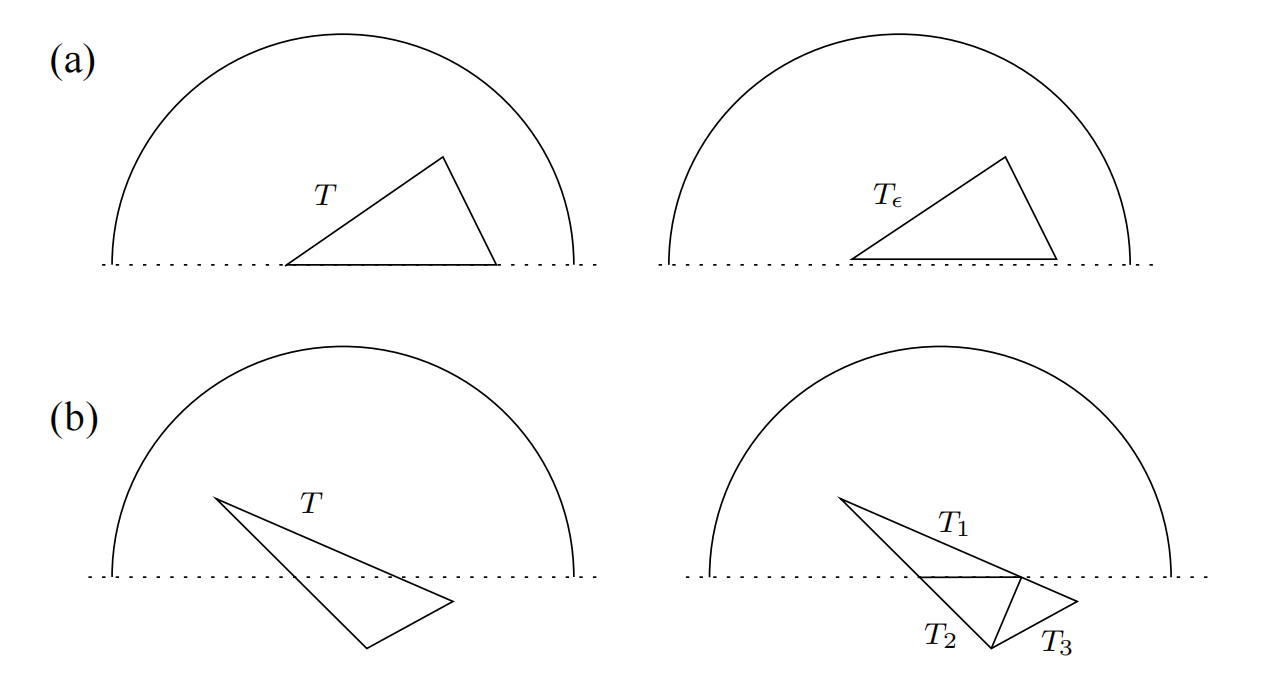
\includegraphics[scale=0.25]{img/proof of Reflection principle.png}
    \caption{(a) Raising a vertex; (b) splitting a triangle}
\end{figure}
\end{center}
Therefore for all $T\subset D_t$, we have 
$$\int_TF(z)\mathrm{d}z=0$$
and hence by Morera's theorem, we have $F$ holomorphic in $\Omega^+\cup L\cup\Omega^-$. This finished the proof.
\end{proof}
The preceding proof gives a traditional proof in the statement that if $f$ is holomorphic on $\Omega\setminus\gamma$, where $\gamma$ is a path, then $f$ is holomorphic on $\Omega$. Another proof, outlined by Rudin, used the property of harmonic functions and we shall introduce below.
\begin{proof}
The only difference is the way to deal with the part on $L$. Let $v(z)=-v(\overline{z})$ for $z\in\Omega^-$. Consider $t\in L$, then by our definition of $v$, it is easily shown that $v$ satisfy the mean value property on $D_t$. Therefore $v$ is harmonic over $D_t$. Now $v$ is the real part for some function $g_t$. Put $f_t=-\mathrm{i}g_t$, then $v$ is the imaginary part of $F$, determined uniquely by $v$ up to a real additive constant. Choose the constant such that $f_t(z)=f(z)$ for some $z\in D_t$. Therefore $f_t(z)=f(z)$ for all $z\in D_t$ since $f-f_t$ is constant in $D_t\cap\Pi^+$, and hence we may define 
$$
F\left( z \right) =\begin{cases}
	f\left( z \right) ,z\in \Omega ^+,\\
	f_t\left( z \right) ,z\in D_t,\\
	\overline{f\left( \overline{z} \right) },z\in \Omega ^-.\\
\end{cases}
$$
The rest proof coincides with the first one.
\end{proof}
\subsection{Boundary Behavior of Possion Integrals}
Our next objective is to find analogous of Theorem 11.2.2 for Poisson integrals of $L^p$-functions and measures on $T$.\par
Let us associate to any function $u$ defined on the unit disc functions $u_r$ on $T$, defined by $u_r(e^{\mathrm{i}\theta})=u(re^{\mathrm{i}\theta})$, here $0\le r<1$. Thus $u_r$ is essentially the restriction of $u$ to the circle with radius $r$, center $0$, but we shift the domain of $u_r$ to $T$.\par
Use this terminology, Theorem 11.2.2 may be stated in the following form: If $f\in C(T)$ and $F=P[f]$, then $F_r\to f$ uniformly on $T$ as $r\to 1$. In other words, 
$$
\lim_{r\rightarrow 1} \left\| F_r-f \right\| =0,
$$
which of course implies 
$$
\lim_{r\rightarrow 1} F_r\left( e^{\mathrm{i}\theta} \right) =f\left( e^{\mathrm{i}\theta} \right) 
$$
at every point of $T$.\par
We shall now develop this result to $L^p$-spaces, and instead of confining ourselves to investigating radial limits, we shall study the nontangential limits of Poisson integrals of measures and $L^p$-functions.
\begin{theorem}
If $1\le p\le\infty$, $f\in L^p(T)$ and $u=P[f]$, then 
$$\|u_r\|_p\le\|f\|_p,\hspace{0.5cm}(0\le r<1)$$
and if $1\le p<\infty$, we have 
$$\lim_{r\to 1}\|u_r-f\|_p=0.$$
\end{theorem}
\begin{proof}
If we apply Jensen's inequality to 
$$
u_r\left( e^{\mathrm{i}\theta} \right) =\frac{1}{2\pi}\int_{-\pi}^{\pi}{f\left( t \right) P_r\left( \theta -t \right) \mathrm{d}t},
$$
we obtain 
$$
\left| u_r\left( e^{\mathrm{i}\theta} \right) \right|^p\le \frac{1}{2\pi}\int_{-\pi}^{\pi}{\left| f\left( t \right) \right|^pP_r\left( \theta -t \right) \mathrm{d}t}.
$$
Therefore by Fubini theorem we have 
$$
\begin{aligned}
\int_{-\pi}^{\pi}{\left| u_r\left( e^{\mathrm{i}\theta} \right) \right|^p\mathrm{d}\theta}&=\frac{1}{2\pi}\int_{-\pi}^{\pi}{\int_{-\pi}^{\pi}{\left| f\left( t \right) \right|^p\cdot P_r\left( \theta -t \right) \mathrm{d}t}\mathrm{d}\theta}
\\
&=\frac{1}{2\pi}\int_{-\pi}^{\pi}{\left| f\left( t \right) \right|^p\mathrm{d}t\int_{-\pi}^{\pi}{P_r\left( \theta -t \right) \mathrm{d}\theta}}
\\
&=\int_{-\pi}^{\pi}{\left| f\left( t \right) \right|^p\mathrm{d}t}.
\end{aligned}
$$
This gives $\|u_r\|_p\le\|f\|_p$. Now to prove the second assertion, put $\varepsilon>0$ an arbitrarily small number. Then there exists some $g\in C(T)$ such that $\|f-g\|_p<\varepsilon$. Let $v=P[g]$, we have 
$$
\left\| u_r-f \right\| _p\le \left\| u_r-v_r \right\| _p+\left\| v_r-g \right\| _p+\left\| g-f \right\| _p\le 2\left\| f-g \right\| _p+\left\| v_r-g \right\| _p\rightarrow 2\varepsilon 
$$
as $r\to 1$, this finished the proof.
\end{proof}
If $\mu$ is a complex measure on $T$, and if we want to replace integrals over $T$ by integrals over intervals of length $2\pi$ in $\mathbb{R}^1$, these intervals have to be taken half open, to avoid possible point masses in $\mu$. Therefore we shall keep integration over circles in what follows, and will write the Poisson integral $u=P[\mathrm{d}\mu]$ of $\mu$ in the form 
$$
u\left( z \right) =\int_T{P\left( z,e^{\mathrm{i}t} \right) \mathrm{d}\mu \left( e^{\mathrm{i}t} \right)}=\int_T{\frac{1-\left| z \right|^2}{\left| e^{\mathrm{i}t}-z \right|^2}\mathrm{d}\mu \left( e^{\mathrm{i}t} \right)},\hspace{0.5cm}z\in U.
$$
Similarly $P[\mathrm{d}\mu]$ is still the real part of a holomorphic function, and hence harmonic in $U$.\par
Setting $\|\mu\|=|\mu|(T)$, then we have $\|\mu_r\|_1\le\|\mu\|$. To see this, note that 
$$
\begin{aligned}
\left\| u_r \right\| _1&=\frac{1}{2\pi}\int_{-\pi}^{\pi}{\left| u\left( re^{\mathrm{i}\theta} \right) \right|\mathrm{d}\theta}=\frac{1}{2\pi}\int_{-\pi}^{\pi}{\left| \int_T{\frac{1-\left| z \right|^2}{\left| e^{\mathrm{i}t}-z \right|^2}\mathrm{d}\mu \left( e^{\mathrm{i}t} \right)} \right|\mathrm{d}\theta}
\\
&\le \frac{1}{2\pi}\int_{-\pi}^{\pi}{\int_T{\left| \frac{1-\left| z \right|^2}{\left| e^{\mathrm{i}t}-z \right|^2} \right|\cdot \mathrm{d}\left| \mu \right|\left( e^{\mathrm{i}t} \right)}\mathrm{d}\theta}=\frac{1}{2\pi}\int_{-\pi}^{\pi}{\left| \frac{1-\left| z \right|^2}{\left| e^{\mathrm{i}t}-z \right|^2} \right|\mathrm{d}\theta \int_T{\mathrm{d}\left| \mu \right|\left( e^{\mathrm{i}t} \right)}}
\\
&=\frac{1}{2\pi}\int_{-\pi}^{\pi}{P_r\left( \theta -t \right) \mathrm{d}\theta}\cdot \left| \mu \right|\left( T \right) =\left\| \mu \right\| .
\end{aligned}
$$\par
For $0<\alpha<1$, we define $\Omega_\alpha$ to be the union of the disc $D(0,\alpha)$ and the line segments from $z=1$ to points of $D(0,\alpha)$ (see figure 4).
\begin{center}
\begin{figure}[htbp]
    \center
    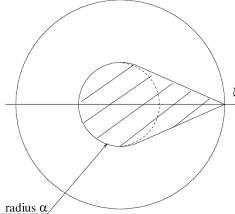
\includegraphics[scale=0.75]{img/nontangential approach region.png}
    \caption{example of a nontangential approach region}
\end{figure}
\end{center}
In other words, $\Omega_\alpha$ is the smallest convex open set that contains $D(0,\alpha)$ and $1$. $\Omega_\alpha$ is called a \textbf{nontangential approach region} with vertex $1$. Trivially $\bigcup_{\alpha}\Omega_\alpha=U$ and $\bigcap_{\alpha}\Omega_\alpha=[0,1)$. By multiplying $e^{\mathrm{i}t}$ on $\Omega_\alpha$, we obtain an rotation of $\Omega_\alpha$, denoted by $e^{\mathrm{i}t}\Omega_\alpha$.\par
If $0<\alpha<1$ and $u$ is any complex function with domain $U$, its \textbf{nontangential maximal function} $N_\alpha$ is defined on $T$ by 
$$
\left( N_{\alpha}u \right) \left( e^{\mathrm{i}t} \right) =\mathrm{sup}\left\{ \left| u\left( z \right) \right|:z\in e^{\mathrm{i}t}\Omega _{\alpha} \right\} .
$$
Similarly, the \textbf{radical maximal function} of $u$ is 
$$
\left( M_{\mathrm{rad}}u \right) \left( e^{\mathrm{i}t} \right) =\mathrm{sup}\left\{ \left| u\left( re^{\mathrm{i}t} \right) \right|:0\le r<1 \right\} .
$$
These maximal functions are easily to see measurable. Consider $\lambda\ge 0$, then both $\left\{ N_{\alpha}u\le \lambda \right\} $ and $\left\{ M_{\mathrm{rad}}u\le \lambda \right\} $ are closed, hence the two functions are lower-semicontinuous.\par
Clearly $M_{\mathrm{rad}}u\le N_\alpha u$ and the latter increases as $\alpha$ increases.\par
We shall introduce some notations now. For convenience, define $\mathrm{d}\sigma=\mathrm{d}m/2\pi$ over $T$. Therefore $\sigma$ is a rotation-invariant Borel measure over $T$ with $\sigma(T)=1$. Accordingly, the maximal function $M\mu$ is now defined by 
$$
M\mu (e^{\mathrm{i}\theta})=\mathrm{sup}\frac{\left| \mu \right|\left( I \right)}{\sigma \left( I \right)},
$$
where the supremum is taken over all arcs $I\subset T$ that centered at $e^{\mathrm{i}\theta}$. Similarly, we have the derivative $D\mu$ of a measure $\mu$ on $T$ 
$$
\left( D\mu \right) \left( e^{\mathrm{i}\theta} \right) =\lim \frac{\mu \left( I \right)}{\sigma \left( I \right)},
$$
as the open arcs shrink to their center $e^{\mathrm{i}\theta}$, and $e^{\mathrm{i}\theta}$ is a \textbf{Lebesgue point} of $f\in L^1(T)$ if 
$$
\lim \frac{1}{\sigma \left( I \right)}\int_I{\left| f-f\left( e^{\mathrm{i}\theta} \right) \right|\mathrm{d}\sigma}=0
$$
with similar $\{I\}$.\par
If $\mathrm{d}\mu=\mathrm{d}\sigma+\mathrm{d}\mu_s$ is the Lebesgue decomposition of a complex Borel measure $\mu$ on $T$ with $\mu_s\perp\sigma$, then by our results in Chapter 7, we have 
$$
\sigma \left\{ M\mu >\lambda \right\} \le \frac{3}{\lambda}\left\| \mu \right\| ,
$$
that almost every point of $T$ is a Lebesgue point of $f$, and that $D\mu=f$, $D\mu_s=0$ a.e. with respect to $\sigma$.\par
We will now see, for any complex Borel measure $\mu$ on $T$, that the nontangential and radial maximal functions of the harmonic function $P[\mathrm{d}\mu]$ are controlled by $M\mu$.
\begin{theorem}
Assume $0<\alpha<1$. Then there exists a constant $c_\alpha>0$ with the following property: If $\mu$ is a positive finite Borel measure on $T$ and $u=P[\mathrm{d}\mu]$ is its Poisson integral, then the inequalities 
$$
c_{\alpha}\left( N_{\alpha}u \right) \left( e^{\mathrm{i}\theta} \right) \le \left( M_{\mathrm{rad}}u \right) \left( e^{\mathrm{i}\theta} \right) \le \left( M\mu \right) \left( e^{\mathrm{i}\theta} \right) 
$$
hold at every point $e^{\mathrm{i}\theta}\in T$.
\end{theorem}
\begin{proof}
We shall prove the condition when $\theta=0$. The general case follows if this special case is applied to the rotation measure $\mu_\theta(E)=\mu(e^{\mathrm{i}\theta}E)$.\par
To prove the first inequality, it suffices to prove that there exists a $c_\alpha$ such that 
$$
c_{\alpha}P\left( z,e^{\mathrm{i}t} \right) \le P\left( \left| z \right|,e^{\mathrm{i}t} \right) .
$$
By the definition of $P(z,e^{\mathrm{i}t})$, it suffices to show that 
$$
c_{\alpha}\left| e^{\mathrm{i}t}-r \right|^2\le \left| e^{\mathrm{i}t}-z \right|^2
$$
with $r=|z|$. By the definition of $\Omega_\alpha$ we have $|z-r|/(1-r)$ is bounded, suppose by $\gamma_\alpha$. Then 
$$
\left| e^{\mathrm{i}t}-r \right|\le \left| e^{\mathrm{i}t}-z \right|+\left| z-r \right|\le \left| e^{\mathrm{i}t}-z \right|+\gamma _{\alpha}\left( 1-r \right) \le \left( 1+\gamma _{\alpha} \right) \left| e^{\mathrm{i}t}-z \right|,
$$
where the last inequality follows from Figure 5. 
\begin{figure}[htbp]
    \center
    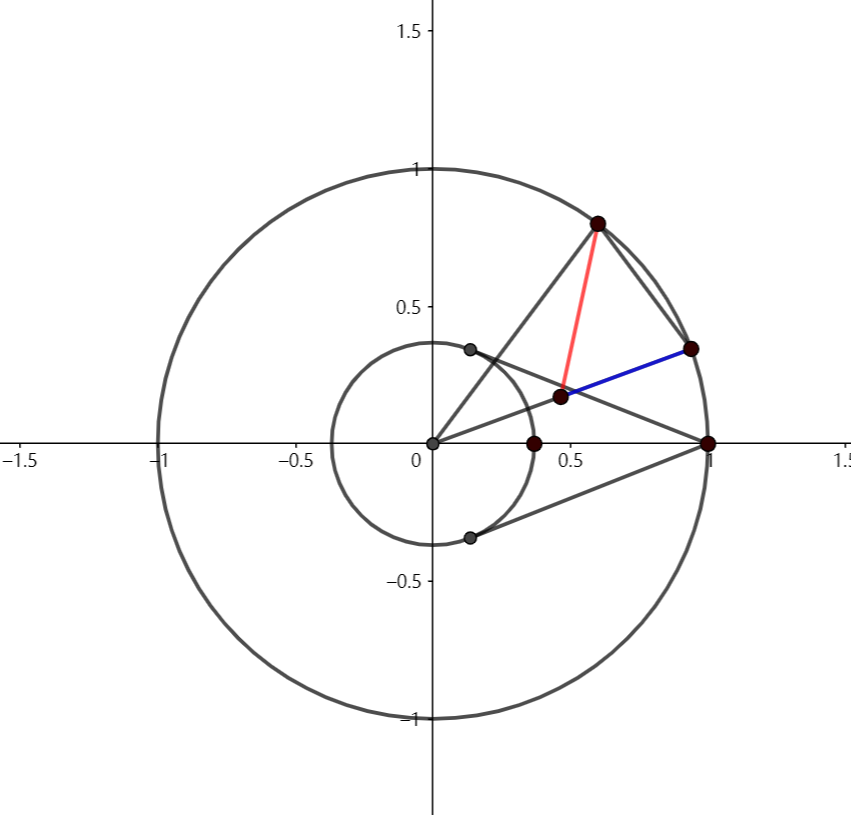
\includegraphics[scale=0.29]{img/proof of an Inequality.png}
    \caption{Geometric Explanation of the Last Inequality}
\end{figure}
Therefore we have 
$$
\frac{1}{\left( 1+\gamma _{\alpha} \right) ^2}\left| e^{\mathrm{i}t}-r \right|^2\le \left| e^{\mathrm{i}t}-z \right|^2
$$
and the proof is finished.\par
For the second inequality, we have to proof that 
$$
\int_T{P_r\left( t \right) \mathrm{d}\mu \left( e^{\mathrm{i}t} \right)}\le \left( M\mu \right) \left( 1 \right) .
$$
Fix $r$. Choose open sets $I_j\subset T$ centered at $1$ such that $I_1\subset I_2\subset\cdots\subset I_{n-1}$. Let $I_n=T$ and $I_0=\emptyset$. Let $\chi_j$ be the characteristic function of the arc $I_j$, let $h_j$ be the largest positive number such that $h_j\chi_j\le P_r$ on $T$. Define 
$$K=\sum_{j=1}^n(h_j-h_{j+1}\chi_j),$$
where $h_{n+1}=0$. Since $P_r(t)$ is an even function of $t$ that decreases as $t$ increase from $0$ to $\pi$, we see that $h_j-h_{j+1}\ge 0$, that $K=h_j$ on $I_j\setminus I_{j-1}$, and $K\le P_r$. The definition of $M\mu$ shows that 
$$\mu(I_j)\le (M\mu)(1)\sigma(I_j),$$
therefore 
$$
\int_T{K\mathrm{d}\mu}=\sum_{j=1}^n{\left( h_j-h_{j+1} \right) \mu \left( I_j \right)}\le M\sum_{j=1}^n{\left( h_j-h_{j+1} \right) \sigma \left( I_j \right)}=M\int_T{K\mathrm{d}\sigma}\le M\int_T{P_r\mathrm{d}\sigma}=M.
$$
Finally, if we choose the arcs $I_j$ so that their endpoints form a sufficiently fine partition of $T$, we obtain step functions $K$ that converges to $P_r$ uniformly on $T$. This finished the proof.
\end{proof}
A function $F$, defined in $U$, is said to \textbf{have nontangential limit} $\lambda$ at $e^{\mathrm{i}\theta}\in T$, if for each $\alpha<1$, 
$$\lim_{j\to\infty}F(z_j)=\lambda$$
for every sequence $\{z_j\}_{i=1}^\infty\subset e^{\mathrm{i}\theta}\Omega_\alpha$ that converges to $e^{\mathrm{i}\theta}$.\par
\begin{theorem}
If $\mu$ is a positive Borel measure on $T$ and $(D\mu)(e^{\mathrm{i}\theta})=0$ for some $\theta$, then its Poisson integral $u=P[\mathrm{d}\mu]$ has nontangential limit $0$ at $e^{\mathrm{i}\theta}$.
\end{theorem}
\begin{proof}
Since $(D\mu)(e^{\mathrm{i}\theta})=0$ for some $\theta$, pick $\varepsilon>0$. There exists some arcs $I_0$ such that $\mu(I)\le\varepsilon\sigma(I)$ for all $I\subset I_0$. Therefore we may divide $\mu$ into two parts, $\mu_0$ being the restriction of $\mu$ over $I_0$, and $\mu_1=\mu-\mu_0$. Define $u_i=P[\mathrm{d}\mu_i]$, where $i=0,1$. Note that 
$$
u_1\left( z_j \right) =\int_{T\setminus I_0}{P\left( z_j,e^{\mathrm{i}t} \right) \mathrm{d}\mu \left( e^{\mathrm{i}t} \right)}=\int_{T\setminus I_0}{\frac{1-\left| z_j \right|^2}{\left| e^{\mathrm{i}t}-z_j \right|^2}\mathrm{d}\mu \left( e^{\mathrm{i}t} \right)}\rightarrow 0,\hspace{0.5cm}\left( j\rightarrow \infty \right) 
$$
and 
$$
u_0\left( z_j \right) \le \left( N_{\alpha}u_0 \right) \left( e^{\mathrm{i}\theta} \right) \le \frac{1}{c_{\alpha}}\left( Mu_0 \right) \left( e^{\mathrm{i}\theta} \right) \le \frac{\varepsilon}{c_{\alpha}},
$$
we have 
$$
\mathop {\lim\mathrm{sup}} \limits_{j\rightarrow \infty}u\left( z_j \right) =\lim_{j\rightarrow \infty} u_0\left( z_j \right) +\mathop {\lim\mathrm{sup}} \limits_{j\rightarrow \infty}u_1\left( z_j \right) \le \frac{\varepsilon}{c_{\alpha}}\rightarrow 0,
$$
this finished the proof.
\end{proof}
\begin{theorem}
If $f\in L^1(T)$, then $P[f]$ has nontangential limit $f(e^{\mathrm{i}\theta})$ at every Lebesgue point $e^{\mathrm{i}\theta}$ of $f$.
\end{theorem}
\begin{proof}
We may suppose $f(e^{\mathrm{i}\theta})=0$, or otherwise subtract a constant from $f$. Then by the definition of a Lebesgue point we have 
$$
\lim \frac{1}{\sigma \left( I \right)}\int_I{\left| f \right|\mathrm{d}\sigma}=0
$$
as the open arcs $I\subset T$ shrink to their center $e^{\mathrm{i}\theta}$. Define a Borel measure $\mu$ on $T$ by 
$$
\mu \left( E \right) =\int_E{\left| f \right|\mathrm{d}\sigma}.
$$
Then we have 
$$
\left( D\mu \right) \left( e^{\mathrm{i}\theta} \right) =\lim \frac{\mu \left( I \right)}{\sigma \left( I \right)}=\lim \frac{1}{\sigma \left( I \right)}\int_I{\left| f \right|\mathrm{d}\sigma}=0,
$$
hence by Theorem 11.4.3 we have $P[\mathrm{d}\mu]$ has nontangential limit $0$ at $e^{\mathrm{i}\theta}$. Note that this is true for $P[f]$ too, since 
$$
\left| P\left[ f \right] \right|\le P\left[ \left| f \right| \right] =P\left[ \mathrm{d}\mu \right] .
$$
This finished the proof.
\end{proof}
The last two theorems can be combined as follows.
\begin{theorem}
If $\mathrm{d}\mu=f\mathrm{d}\sigma+\mathrm{d}\mu_s$ is the Lebesgue decomposition of a complex Borel measure $\mu$ on $T$, where $f\in L^1(T)$, $\mu_s\perp\sigma$, then $P[\mathrm{d}\mu]$ has nontangential limit $f(e^{\mathrm{i}\theta})$ at almost every point of $T$.
\end{theorem}
\begin{proof}
Since $\mu_s$ is a complex Borel measure such that $\mu_s\perp\sigma$, by Theorem 7.1.10 we have $(D\mu_s)(e^{\mathrm{i}\theta})=0$ and hence by Theorem 11.4.3 we have $P[\mathrm{d}\mu_s]$ has nontangential limit $0$ at $e^{\mathrm{i}\theta}$. Since almost every point on $T$ is a Lebesgue point of $f$, apply Theorem 11.4.4 to finish the proof.
\end{proof}
Here is another consequence of Theorem 11.4.2.
\begin{theorem}
For $0<\alpha<1$ and $1\le p\le\infty$, there are constants $A(\alpha,p)<\infty$ with the following properties: \par
(a) If $\mu$ is a complex Borel measure on $T$, and $u=P[\mathrm{d}\mu]$, then 
$$
\sigma \left\{ N_{\alpha}u>\lambda \right\} \le \frac{A\left( \alpha ,1 \right)}{\lambda}\left\| \mu \right\| .\hspace{0.5cm}\left( 0<\lambda <\infty \right) 
$$\par
(b) If $1<p\le\infty$, $f\in L^p(T)$ and $u=P[f]$, then 
$$
\left\| N_{\alpha}u \right\| _p\le A\left( \alpha ,p \right) \left\| f \right\| _p.
$$
\end{theorem}
\begin{proof}
(a) By Theorem 7.1.3 and Theorem 11.4.2 we have 
$$
\sigma \left\{ N_{\alpha}u>\lambda \right\} =\sigma \left\{ c_{\alpha}\left( N_{\alpha}u \right) >c_{\alpha}\lambda \right\} \le \sigma \left\{ M_{\alpha}u>c_{\alpha}\lambda \right\} \le \frac{3^k}{c_{\alpha}\lambda}\left\| \mu \right\| .
$$\par
(b) By Theorem 8.6.2 and Theorem 11.4.2 we have 
$$
\left\| N_{\alpha}u \right\| _p=\frac{1}{c_{\alpha}}\left\| c_{\alpha}\left( N_{\alpha}u \right) \right\| _p\le \frac{1}{c_{\alpha}}\left\| M_{\alpha}u \right\| _p\le \frac{c_p}{c_{\alpha}}\left\| f \right\| _p,
$$
which finished the proof.
\end{proof}
Thus the nontangential maximal function of $u$ is in weak $L^1$ if $u=P[\mathrm{d}\mu]$, and they are in $L^p$ if $u=P[f]$ for some $f\in L^p(T)$, $p>1$.
\subsection{Representation Theorems}
How can we tell whether a harmonic function $u$ in $U$ is a Poisson integral or not? The preceding theorems contain a number of necessary conditions. It turns out that the simplest of these, the $L^p$-boundedness of the family $\{u_r:0\le r<1\}$ is also sufficient. Thus, in particular, the boundedness of $\|u_r\|_1$ as $r\to 1$ implies the existence of nontangential limits a.e. on $T$, since, as we will see, $u$ can be represented as the Poisson integral of a measure.\par
This measure will be obtained as a so-called "weak limit" of the functions $u_r$. Weak convergence is an important topic in functional analysis. We will approach it through another important concept, called equicontinuity, which we will meet again later, in connection with the so-called "normal families" of holomorphic functions.
\begin{definition}
Let $\mathscr{F}$ be a collection of complex functions on a metric space $X$ with metric $\rho$.\par
We say that $\mathscr{F}$ is \textbf{equicontinuity} if to every $\varepsilon>0$ corresponds a $\delta>0$ such that $|f(x)-f(y)|<\varepsilon$ for every $f\in\mathscr{F}$ and for all pairs of points $x,y$ with $\rho(x,y)<\delta$.
\end{definition}
It is known that $\mathscr{F}$ is a class of functions that are equicontinuous and pointwise bounded is equivalent to say that $\mathscr{F}$ is countably compact. This is the so-called \textbf{Arzela-Ascoli Theorem}.
\begin{theorem}
Suppose that \par
(a) $X$ is a separable Banach space,\par
(b) $\{\Lambda_n\}$ is a sequence of linear functionals on $X$,\par
(c) $\sup_n\|\Lambda_n\|=M<\infty$.\par
Then there is a subsequence $\{\Lambda_{n_i}\}$ such that the limit 
$$\Lambda x=\lim_{i\to\infty}\Lambda_{x_i}x$$
exists for every $x\in X$. Moreover, $\Lambda$ is linear, and $\|\Lambda\|\le M$.
\end{theorem}
\begin{proof}
Since $X$ is separable, it suffices to show that $\Lambda_n$ is bounded pointwise and equicontinuous. Now observe that $|\Lambda_nx|\le M\|x\|$ for all $x\in X$ and 
$$
\left| \Lambda _nx^{\prime}-\Lambda _nx^{\prime\prime} \right|\le M\cdot \left\| x^{\prime}-x^{\prime\prime} \right\| ,
$$
we have $\{\Lambda_n\}$ is bounded pointwise and equicontinuous. Hence there exists a subsequence $\{\Lambda_{n_i}\}$ such that $\Lambda_{n_i}\to\Lambda$ for some $\|\Lambda\|\le M$.
\end{proof}
Recall that $C(T)$ and $L^p(T)$ is separable since the trigonometric series are dense in them. We have the following representation theorem: 
\begin{theorem}
Suppose $u$ is harmonic in $U$, $1\le p\le\infty$ and 
$$\sup_{0<r<1}\|u_r\|_p=M<\infty.$$\par
(a) If $p=1$, it follows that there is a unique complex Borel measure $\mu$ on $T$ so that $u=P[\mathrm{d}\mu]$.\par
(b) If $p>1$, it follows that there is a unique $f\in L^p(T)$ so that $u=P[f]$.\par
(c) Every positive harmonic function in $U$ is the Poisson integral of a unique positive Borel measure on $T$.
\end{theorem}
\begin{proof}
We shall first prove (a) and (b). For existence, we define 
$$
\Lambda _rg=\int_T{u_rg\mathrm{d}\sigma}.\hspace{0.5cm}\left( 0\le r<1 \right) 
$$
It follows that $\|\Lambda_r\|\le M$ since 
$$
\left\| \Lambda _r \right\| =\mathop {\mathrm{sup}} \limits_{g\in L^p\left( U \right) \setminus \left\{ 0 \right\}}\frac{\left\| \Lambda _rg \right\|}{\left\| g \right\| _p}\le \mathop {\mathrm{sup}} \limits_{g\in L^p\left( U \right) \setminus \left\{ 0 \right\}}\frac{\left\| \Lambda _r \right\| \cdot \left\| g \right\| _p}{\left\| g \right\| _p}\le \mathop {\mathrm{sup}} \limits_{0\le r<1}\left\| u_r \right\| _p\le M.
$$
Now if $p=1$, by Theorem 11.5.2 and the complex version of Riesz Representation Theorem we have 
$$
\lim_{j\rightarrow \infty} \int_T{g\cdot u_{r_j}\mathrm{d}\sigma}=\int_T{g\mathrm{d}\mu}
$$
for some complex Borel measure $\mu$ with $\|\mu\|\le M$ and a sequence $r_j\to 1$. Define $h_j(z)=u(r_jz)$, we have $h_j$ a harmonic function in $U$ and continuous on $\overline{U}$. Therefore 
$$
h_j\left( z \right) =\int_T{P\left( z,e^{\mathrm{i}t} \right) h_j\left( e^{\mathrm{i}t} \right) \mathrm{d}\sigma \left( e^{\mathrm{i}t} \right)}.
$$
Hence for $g(e^{\mathrm{i}t})=P(z,e^{\mathrm{i}t})$, we have 
$$
u\left( z \right) =\lim_{j\rightarrow \infty} u\left( r_jz \right) =\lim_{j\rightarrow \infty} h_j\left( z \right) =\lim_{j\rightarrow \infty} \int_T{P\left( z,e^{\mathrm{i}t} \right) h_j\left( e^{\mathrm{i}t} \right) \mathrm{d}\sigma \left( e^{\mathrm{i}t} \right)}=\int_T{P\left( z,e^{\mathrm{i}t} \right) \mathrm{d}\mu \left( e^{\mathrm{i}t} \right)}=P\left[ \mathrm{d}\mu \right] \left( z \right) .
$$
For $p>1$, suppose $q$ is the conjugate exponent of $p$, then $L^q(T)$ is separable. Therefore by the representation of linear functionals in $L^p$ spaces, there exists some $f\in L^p$ and $r_j\to 1$ such that 
$$
\lim_{j\rightarrow \infty} \int_T{g\cdot u_{r_j}\mathrm{d}\sigma}=\int_T{fg\mathrm{d}\sigma}.
$$
Now define $h_j$ in an analogous way and we obtain 
$$
u\left( z \right) =\int_T{P\left( z,e^{\mathrm{i}t} \right) f\left( e^{\mathrm{i}t} \right) \mathrm{d}\sigma \left( e^{\mathrm{i}t} \right)}=P\left[ f \right] \left( z \right) .
$$
To prove the uniqueness, it suffices to show that $P[\mathrm{d}\mu]=0$ implies $\mu=0$. Pick $f\in C(T)$, $u=P[f]$ and $v=P[\mathrm{d}\mu]$. Then 
$$
\begin{aligned}
\int_T{u_r\mathrm{d}\mu}&=\int_T{\left( \int_T{P\left( re^{\mathrm{i}\theta},e^{\mathrm{i}t} \right) f\left( e^{\mathrm{i}t} \right) \mathrm{d}\sigma \left( e^{\mathrm{i}t} \right)} \right) \mathrm{d}\mu}
\\
&=\int_T{\left( \int_T{P\left( re^{\mathrm{i}t},e^{\mathrm{i}\theta} \right) f\left( e^{\mathrm{i}t} \right) \mathrm{d}\sigma \left( e^{\mathrm{i}t} \right)} \right) \mathrm{d}\mu}
\\
&=\int_T{f\left( e^{\mathrm{i}t} \right) \mathrm{d}\sigma \left( e^{\mathrm{i}t} \right) \int_T{P\left( re^{\mathrm{i}t},e^{\mathrm{i}\theta} \right) \mathrm{d}\mu \left( e^{\mathrm{i}\theta} \right)}}
\\
&=\int_T{f\left( e^{\mathrm{i}t} \right) \mathrm{d}\sigma \left( e^{\mathrm{i}t} \right) \int_T{P\left( re^{\mathrm{i}t},e^{\mathrm{i}\theta} \right) \mathrm{d}\mu \left( e^{\mathrm{i}\theta} \right)}}=\int_T{v_rf\mathrm{d}\sigma}.
\end{aligned}
$$
When $v=0$ then $v_r=0$, and since $u_r\to f$ uniformly, as $r\to 1$, we have $\int_Tf\mathrm{d}\mu=0$. This implies $\mu=0$.\par
Finally (c) is a corollary of (a), since $u>0$ implies 
$$
\left\| u_r \right\| _1=\int_T{\left| u_r \right|\mathrm{d}\sigma}=\int_T{u_r\mathrm{d}\sigma}=u_r\left( 0 \right) =u\left( 0 \right) >0,
$$
therefore the linear functionals $\Lambda_r$ are positive and hence $\mu\ge 0$.
\end{proof}
Since holomorphic functions are harmonic, all of our preceding results apply to holomorphic functions in $U$. This leads us to study $H^p$-spaces, which we shall discuss in the future sections.\par
At present we shall only give one application, to functions in the space $H^\infty$. This, by definition, is the space of all bounded holomorphic functions in $U$, the norm 
$$\|f\|_\infty=\sup\{|f(z)|:z\in U\}$$
turn $H^\infty$ into a Banach space.
\begin{theorem}
To every $f\in H^\infty$ corresponds a function $f^*\in L^\infty(T)$, defined almost everywhere by 
$$f^*(e^{\mathrm{i}\theta})=\lim_{r\to 1}f(re^{\mathrm{i}\theta}).$$
The equality $\|f\|_\infty=\|f^*\|_\infty$ holds.\par
If $f^*(e^{\mathrm{i}\theta})=0$ for almost all $e^{\mathrm{i}\theta}$ on some arc $I\subset T$, then $f(z)=0$ for every $z\in U$.
\end{theorem}
\begin{proof}
By Theorem 11.5.3 we know that there exists some $g\in L^\infty(U)$ such that $f=P[g]$. Therefore $g$ satisfies $f(re^{\mathrm{i}\theta})\to g(e^{\mathrm{i}\theta})$. Now we show that $\|f\|_\infty=\|g\|_\infty$. Indeed we have 
$$
\left\| f \right\| _{\infty}=\left\| P\left[ g \right] \right\| _{\infty}\le \left\| g \right\| _{\infty}\cdot \int_T{P\left( z,e^{\mathrm{i}t} \right) \mathrm{d}\sigma \left( e^{\mathrm{i}t} \right)}=\left\| g \right\| _{\infty}\le \left\| f \right\| _{\infty},
$$
where the last equality follows from the limit process.\par
Now suppose $f^*(e^{\mathrm{i}\theta})=0$ for almost all $e^{\mathrm{i}\theta}$ on some arc $I\subset T$, then we may choose some $n\in\mathbb{Z}$ such that $|I|>2\pi/n$. Therefore define 
$$
F\left( z \right) =\prod_{k=1}^n{f\left( e^{\mathrm{i}\cdot \frac{2k\pi}{n}}\cdot z \right)},\hspace{0.5cm}\left( z\in U \right) 
$$
we have $F\in H^\infty(U)$ and $F^*=0$ a.e. on $T$, hence $\|F\|_\infty=0$ and $F(z)=0$ for all $z\in U$. Now suppose $Z(f)$ be the set of all zeros of $f$, then 
$$
Z\left( F \right) =\bigcup_{k=1}^n{Z\left( e^{\mathrm{i}\cdot \frac{2k\pi}{n}}\cdot f \right)}
$$
is a union of rotations of zeros of $f$, which is uncountable. Therefore $Z(f)$ is uncountable and hence $f=0$ for all $z\in U$.
\end{proof}
\subsection{Exercises for Chapter XI}
\begin{problem}\em
Suppose $u$ and $v$ are real harmonic functions in a plane region $\Omega$. Under what circumstances is $uv$ harmonic? For which $f\in H(\Omega)$ is $|f|^2$ harmonic?
\end{problem}
\begin{proof}
We first claim that $uv$ is harmonic if and only if $u_xv_x+u_yv_y=0$. This follows from a simple calculation that 
$$
\begin{aligned}
\Delta \left( uv \right) &=\left( u_xv+uv_x \right) _x+\left( u_yv+uv_y \right) _y
\\
&=v\cdot \Delta u+u\cdot \Delta v+2\left( u_xv_x+u_yv_y \right) 
\\
&=2\left( u_xv_x+u_yv_y \right) .
\end{aligned}
$$
Therefore $uv$ is harmonic if and only if $u_xv_x+u_yv_y=0$.\par
Now suppose $f=u+\mathrm{i}v$. Then $|f|^2=u^2+v^2$. We first claim that $u^2$ is harmonic if and only if $u$ is a constant. Note that 
$$
\begin{aligned}
\Delta \left( u^2 \right) &=\left( 2u\cdot u_x \right) _x+\left( 2u\cdot u_y \right) _y
\\
&=2\left( u_{x}^{2}+u\cdot u_{xx} \right) +2\left( u_{y}^{2}+u\cdot u_{yy} \right) 
\\
&=2\left( u_{x}^{2}+u_{y}^{2}+u\cdot \Delta u \right) 
\\
&=2\left( u_{x}^{2}+u_{y}^{2} \right) ,
\end{aligned}
$$
we therefore obtain $\Delta(u^2)=0$ if and only if $u$ is a constant. This implies $|f|^2$ harmonic if and only if $f$ is a constant.
\end{proof}
\begin{problem}\em
If $u$ is a harmonic function in a region $\Omega$, what can you say about the set of points at which the gradient of $u$ is zero?
\end{problem}
\begin{proof}
Define $V=\{x\in\Omega:\nabla u(x)=0\}$. Then we consider $f=u_x+\mathrm{i}u_y$, clearly the zeros of $f$, denoted as $Z(f)$, is the same as $V$. Therefore $Z(f)=V$ is either equal to $\Omega$ or has only countably many points in it. If $Z(f)=\Omega$, then $f$ is a constant, hence $u$ is also a constant. Otherwise $Z(f)$ consists of only countably many points and has no limit points.
\end{proof}
\begin{problem}\em
Suppose $f\in H(\Omega)$ and $|f|$ has no zeros. Prove that $\log|f|$ is harmonic in $\Omega$.
\end{problem}
\begin{proof}
We proof with a direct computation. Note that 
$$
\begin{aligned}
\Delta \left( \log \left| f \right| \right) &=\frac{\partial}{\partial x}\left( \frac{\partial}{\partial x}\log \left| f \right| \right) +\frac{\partial}{\partial y}\left( \frac{\partial}{\partial y}\log \left| f \right| \right) 
\\
&=\frac{\partial}{\partial x}\left( \frac{u\cdot u_x+v\cdot v_x}{u^2+v^2} \right) +\frac{\partial}{\partial y}\left( \frac{u\cdot u_y+v\cdot v_y}{u^2+v^2} \right) 
\\
&=\frac{\left( u^2+v^2 \right) \left[ \left( u_{x}^{2}+u_{y}^{2} \right) +\left( v_{x}^{2}+v_{y}^{2} \right) \right]}{\left( u^2+v^2 \right) ^2}-\frac{\left( u_{x}^{2}+u_{y}^{2} \right) +\left( v_{x}^{2}+v_{y}^{2} \right)}{u^2+v^2}
\\
&=\frac{\left( u_{x}^{2}+u_{y}^{2} \right) +\left( v_{x}^{2}+v_{y}^{2} \right)}{u^2+v^2}-\frac{\left( u_{x}^{2}+u_{y}^{2} \right) +\left( v_{x}^{2}+v_{y}^{2} \right)}{u^2+v^2}=0.
\end{aligned}
$$
Hence $\log|f|$ is harmonic.
\end{proof}
\begin{problem}\em
Suppose $f\in H(U)$, where $U$ is the open unit disc, $f$ is one-to-one in $U$, $\Omega=f(U)$ and $f(z)=\sum c_nz^n$. Prove that the area of $\Omega$ is $\pi\sum n|c_n|^2$.
\end{problem}
\begin{proof}
Note that the Jacobian of $f$ is 
$$
\mathrm{Jac}\left( f \right) =\left| \frac{\partial \left( u,v \right)}{\partial \left( x,y \right)} \right|=\mathrm{abs} \left( \left| \begin{matrix}
	u_x&		u_y\\
	v_x&		v_y\\
\end{matrix} \right| \right) =\mathrm{abs} \left( u_xv_y-v_xu_y \right) =\left| f^{\prime} \right|^2,
$$
we therefore obtain 
$$
\begin{aligned}
S\left( \Omega \right) &=\iint_{\Omega}{\mathrm{d}x\mathrm{d}y}=\iint_U{\left| f^{\prime}\left( z \right) \right|\mathrm{d}x\mathrm{d}y}=\iint_U{f^{\prime}\left( z \right) \cdot \overline{f^{\prime}\left( z \right) }\mathrm{d}x\mathrm{d}y}
\\
&=\int_0^{2\pi}{\int_0^1{f^{\prime}\left( r\cos \theta ,r\sin \theta \right) \cdot \overline{f^{\prime}\left( r\cos \theta ,r\sin \theta \right) }\cdot r\mathrm{d}r\mathrm{d}\theta}}
\\
&=\int_0^{2\pi}{\int_0^1{\left( \sum_{n=1}^{\infty}{nc_n\cdot r^{n-1}e^{\mathrm{i}\left( n-1 \right) \theta}} \right) \cdot \left( \sum_{m=1}^{\infty}{m\overline{c_m}\cdot r^{m-1}e^{-\mathrm{i}\left( m-1 \right) \theta}} \right) \cdot r\mathrm{d}r\mathrm{d}\theta}}
\\
&=\int_0^{2\pi}{\int_0^1{\sum_{n=1}^{\infty}{\sum_{m=1}^{\infty}{nm\cdot c_n\overline{c_m}\cdot r^{n+m-1}e^{\mathrm{i}\left( n-m \right) \theta}}}\mathrm{d}r}\mathrm{d}\theta}
\\
&=\int_0^{2\pi}{\int_0^1{\sum_{n=1}^{\infty}{n^2\left| c_n \right|^2\cdot r^{2n-1}\mathrm{d}r\mathrm{d}\theta}}}
\\
&=\int_0^{2\pi}{\left( \sum_{n=1}^{\infty}{\int_0^1{n^2\left| c_n \right|^2\cdot r^{2n-1}\mathrm{d}r}} \right) \mathrm{d}\theta}
\\
&=2\pi \sum_{n=1}^{\infty}{n^2\left| c_n \right|^2\cdot \frac{1}{2n}}=\pi \sum_{n=1}^{\infty}{n\left| c_n \right|^2},
\end{aligned}
$$
where we now examine the procedure of interchanging sum and integrals. Since $f\in H(U)$, we have 
$$
f^{\prime}\left( z \right) =\sum_{n=1}^{\infty}{nc_n\cdot z^{n-1}}\in H\left( U \right) 
$$
and hence 
$$
\mathop {\lim\mathrm{sup}} \limits_{n\rightarrow \infty}\sqrt[n]{n^2\left| c_n \right|^2}=\mathop {\lim\mathrm{sup}} \limits_{n\rightarrow \infty}\sqrt[n]{n\cdot \left| c_n \right|}=1.
$$
This finished the proof.
\end{proof}